\chapter{Design}
\section*{Overview}
This section includes a breakdown of the application into sections of data processing, GUI functionalities and joint functionalities. The use of external sources including DM-D.S.S. and NIED data sources is discussed, together with the relevant formats (JSON) and the objects related. UML class diagrams are included to discuss OOP relations of classes, records (record classes) and enums including the use of inheritance, composition, association and aggregation. They also implement different interfaces. Design patterns that should be included in the application are also introduced and outlined. An outline of the design of the user interface is included. The expected hardware requirements of the systems are also listed, but any laptop with an up-to-date operating system (running Windows or macOS) should be able to run the program.

\section{Hierarchy Chart}
As discussed in the analysis section, the program consists of three parts: data-parsing from external data sources, GUI functionalities and joint functionalities, where the GUI part will be divided into two parts focusing on real-time monitoring and past-earthquake information, respectively. Here, functionalities for each particular module is further split up. Figure \ref{fig:hierarchy} is a hierarchy diagram for the whole application. This shows how \textbf{decomposition} technique is applied to reduce a sophisticated problem into more attackable problems.

\begin{figure}[htp]
    \centering
    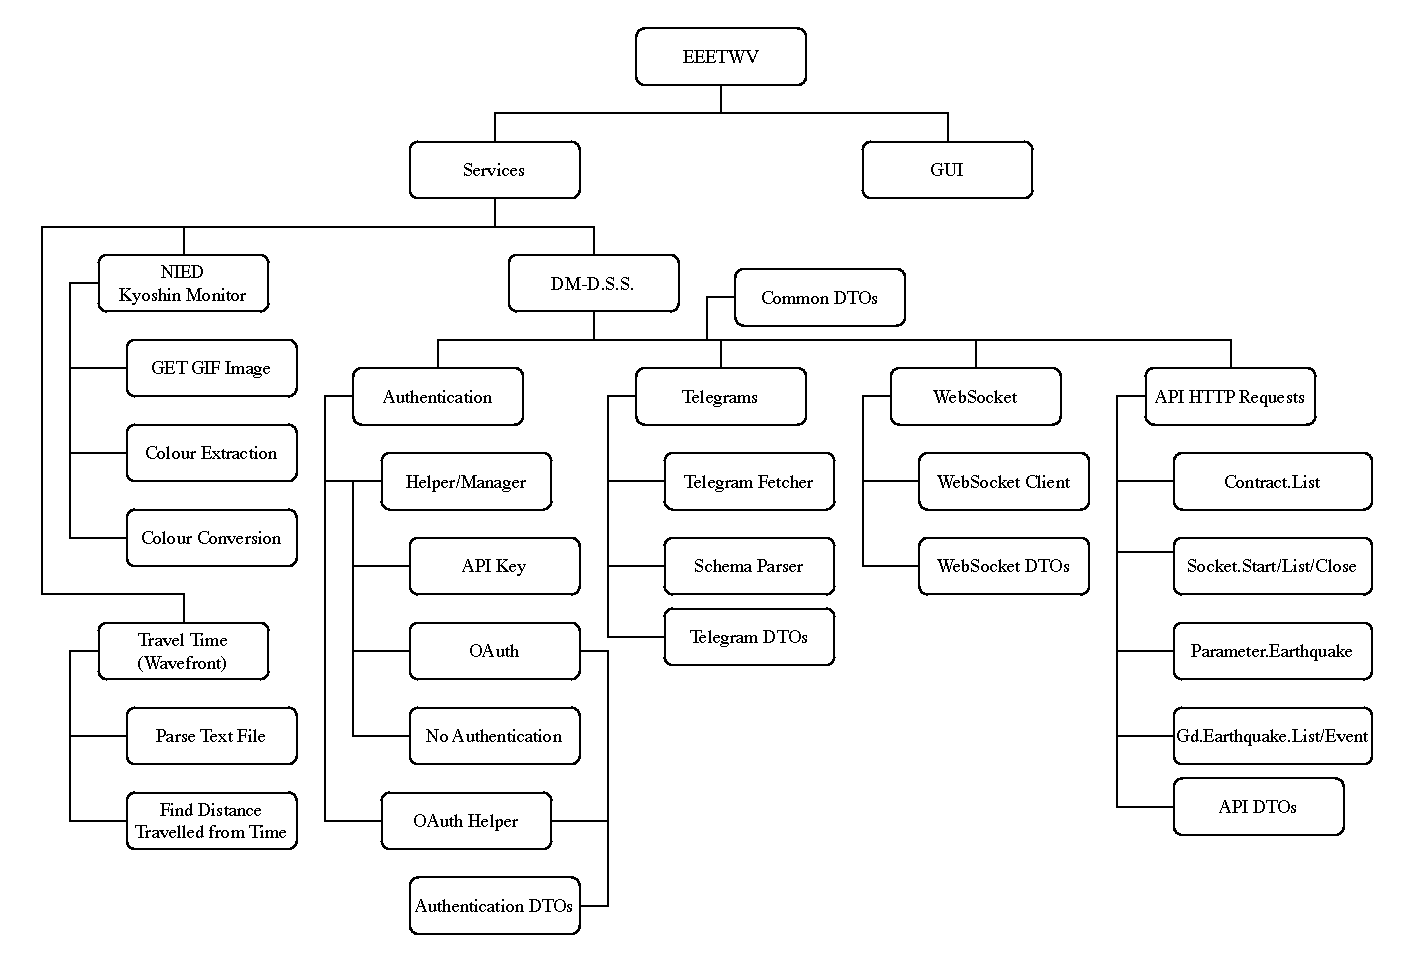
\includegraphics[width=\linewidth]{hierarchy.pdf}
    \caption{Hierarchy chart of the whole application}
    \label{fig:hierarchy}
\end{figure}

Since the GUI part is quite complicated, it is included in this separate diagram, in Figure \ref{fig:hierarchy-gui}.

\begin{figure}[htp]
    \centering
    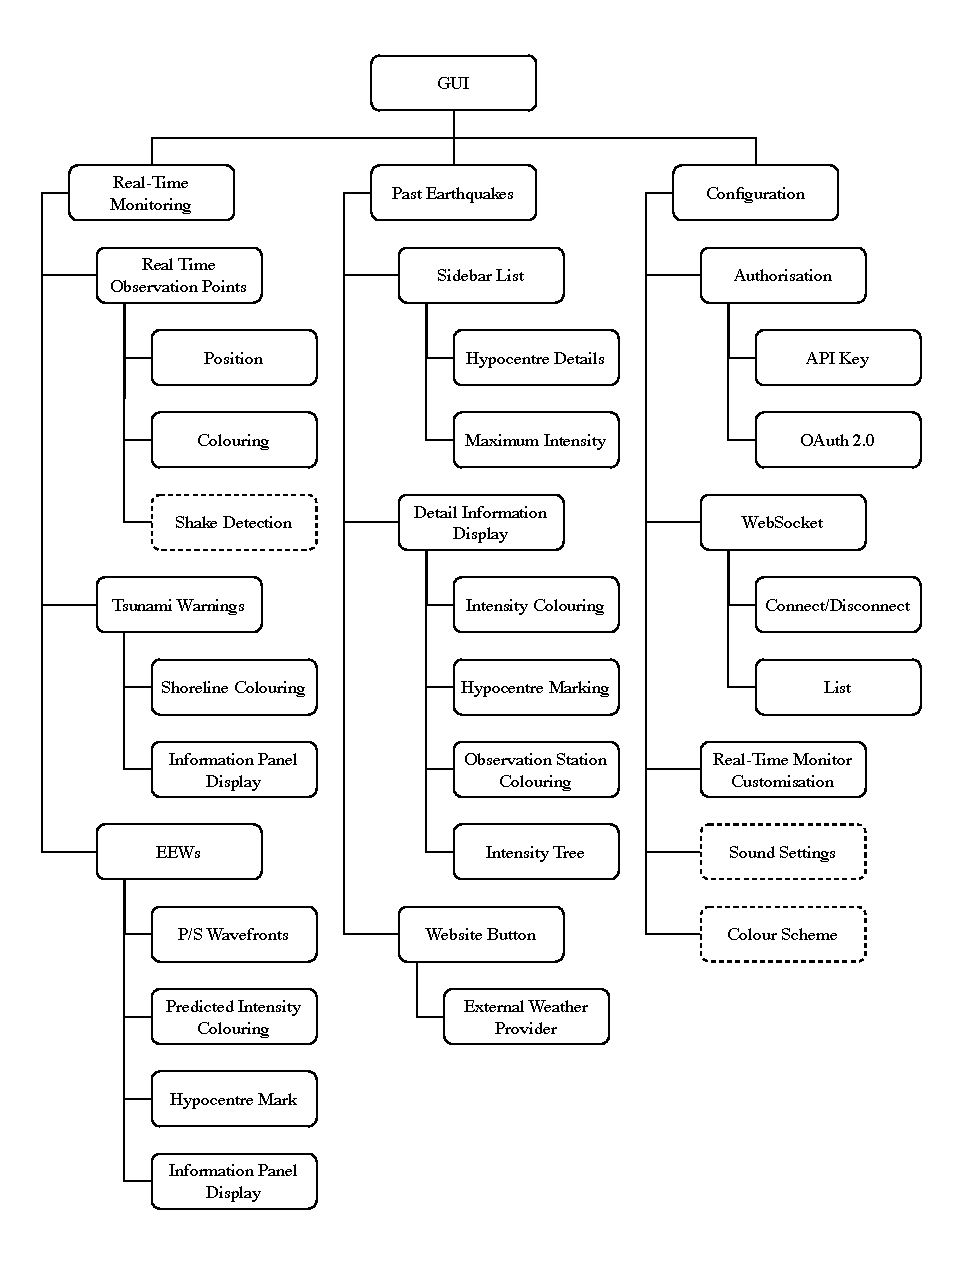
\includegraphics[width=0.8\linewidth]{hierarchy-gui.pdf}
    \caption{Hierarchy chart of the GUI Component}
    \label{fig:hierarchy-gui}
\end{figure}

The whole application (apart from the polynomial fitting part which was done in Python) will be written in C\# using the .NET Core Version 9.0, since the .NET Core is designed oriented around OOP techniques, and some JSON properties (e.g. the \Code{JsonStringEnumMemberName} to customise the parsing of enums) will require the use of .NET 9.

\section{External Data Sources}
There are two data sources this program will use: the NIED and the DM-D.S.S. Specifically, the former one is used to achieve the real-time shake data of the sensor points which were set up by the government (whose data is free to use), and the latter one is used to achieve past earthquake information and EEW information sent out by the JMA (which is pay-to-use). Note that DM-D.S.S. does also provide the real-time intensity data of the observation points, however it is pay-to-use only for companies and institutions on request. Therefore, it will not be feasible to use this data source in the program since one of and the principle target users is people passionate in monitoring earthquakes.

\subsection{NIED Data Source}

As mentioned before, NIED has numerous 'earthquake observation nets' across Japan. Specifically, there is the K-NET and KiK-net \autocite{nied-k-kik-net}, which is dedicated to the observation of strong seismic motion. The K-NET consists of approximately 1000 sensors located across Japan, while the KiK-net also includes some sensors which are located within the earth, which will often have different readings compared to those located on the surface. They are extremely capable of detecting strong motion of ground. Furthermore, the K-NET and the KiK-net provides real-time intensity data webpage of two types, the \href{http://www.kmoni.bosai.go.jp}{'Kyoshin' (強震) monitor} and the \href{https://www.lmoni.bosai.go.jp/monitor/}{long-period ground motion (LPGM, 長周期地震動) monitor} (not working at the time of investigation). The Hi-net \autocite{nied-hi-net} stands for high-sensitivity seismograph network, and it is dedicated for observation of minor motions of the ground. They release the waveforms to those who are researching seismic movements. As for the F-net \autocite{nied-f-net} which stands for the Full Range Seismograph Network of Japan, which is used to analyse the mechanism of a certain earthquake by analysing movements. None of the three nets provide a real-time API data feed.

Having compared the functionalities described above of the K/KiK-net, Hi-net and F-net and how they feed the data sources, the most suitable data source to reflect real-time motion of ground movements will be the \textbf{K/KiK-net}'s data feed, since it detects strong ground movements and is available real-time for the purpose of the application. (This is also the data source that JQuake and KEVI use in fact.)

In fact, in addition to these three networks, there are also the S-net, the DONET and the N-net, which detects the ground seismic movements in the sea. These data were adapted by SREV, but this is beyond the scope of this NEA analysis.

A comparison from the official website of MOWLAS (Monitoring of Waves on Land and Seafloor) \autocite{nied-mowlas} of the three nets are included in Figure \ref{fig:net-comparison} and a map of the distribution of the sensors are included in Figure \ref{fig:net-distribution}.

\begin{figure}[htp]
    \centering
    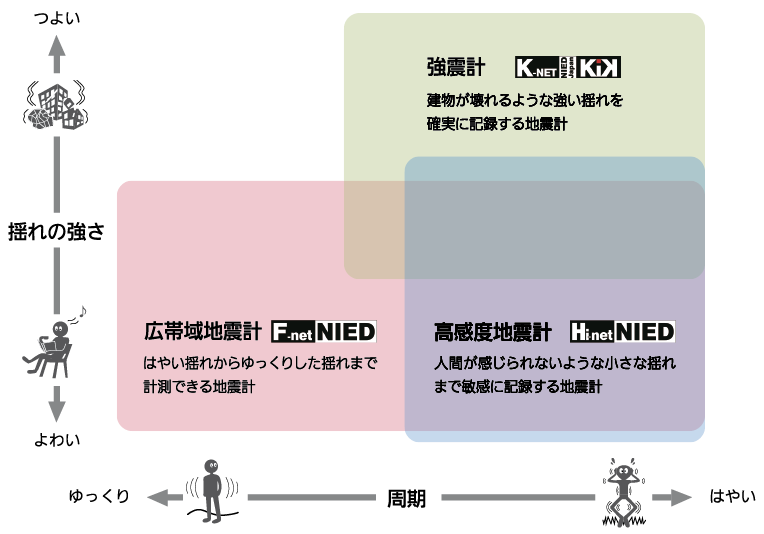
\includegraphics[width=0.75\linewidth]{net-comparison.png}
    \caption{A comparison of the K-NET, F-net and Hi-net.}
    \label{fig:net-comparison}
\end{figure}

\begin{figure}[htp]
    \centering
    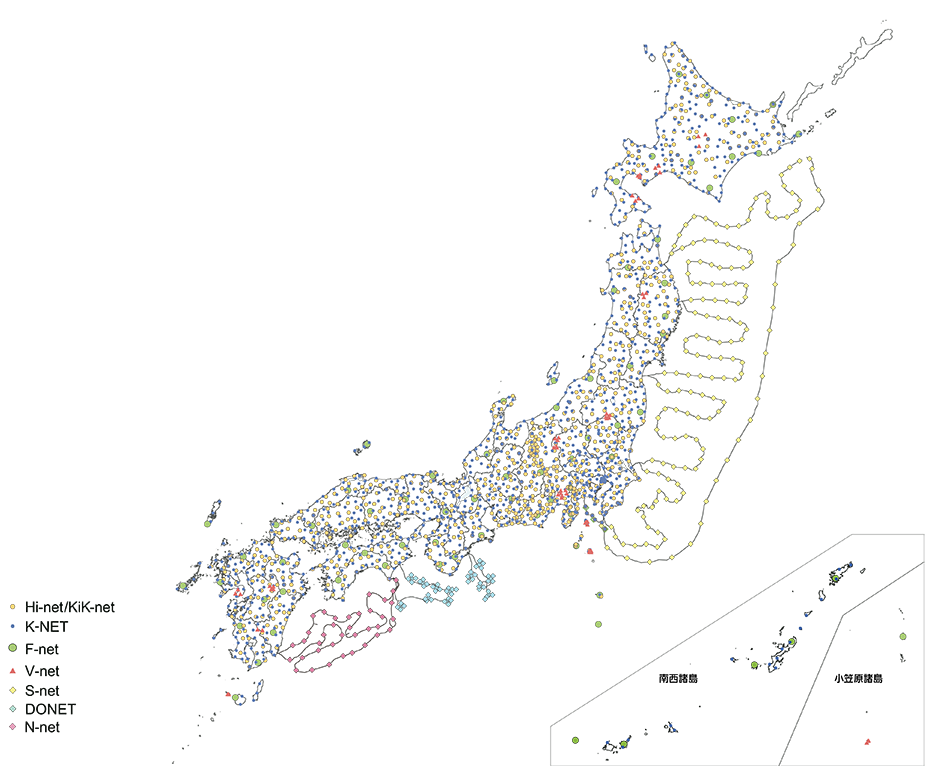
\includegraphics[width=0.75\linewidth]{net-distribution.png}
    \caption{Distribution of the sensors of different nets.}
    \label{fig:net-distribution}
\end{figure}

\subsubsection{Achieving image format data source}

The data source fed by the 'Kyoshin' Monitor is split into 8 types (detailed below in Table \ref{tab:kmoni-data-types}), and each type split into 2 types of data sources, surface sensors and borehole (earth) sensors, with codes in Table \ref{tab:kmoni-sensor-types}. The link to the GIF image is in the following format:

\begin{center}
    \url{http://www.kmoni.bosai.go.jp/data/map_img/RealTimeImg/[#1]_[#2]/[yyyyMMdd]/[yyyyMMdd][hhmmss].[#1]_[#2].gif}
\end{center}

In the link, the \Code{[yyyyMMdd]} and the \Code{[hhmmss]} part should be replaced with the date and time respectively (in JST, UTC+8), and the \Code{#1} replaced with the codes detailed below for the data types, and \Code{#2} replaced with the codes detailed below for data sources. An example of the imaged achieved is in Figure \ref{fig:sample-kmoni}.

\begin{table}[htp]
    \centering

    \begin{tabular}{ccc}
        Data Type        & Description/Meaning                & Code in \Code{#1} \\
        \hline
        Real-time Shindo & Real-time Measured Intensity       & \Code{jma}        \\
        PGA              & Peak (Maximal) Ground Acceleration & \Code{acmap}      \\
        PGV              & Peak (Maximal) Ground Velocity     & \Code{vcmap}      \\
        PGD              & Peak (Maximal) Ground Displacement & \Code{dcmap}      \\
        Response 0.125Hz & Response spectrum for 0.125Hz PGV  & \Code{rsp0125}    \\
        Response 0.250Hz & Response spectrum for 0.250Hz PGV  & \Code{rsp0250}    \\
        Response 0.500Hz & Response spectrum for 0.500Hz PGV  & \Code{rsp0500}    \\
        Response 1.000Hz & Response spectrum for 1.000Hz PGV  & \Code{rsp1000}    \\
        Response 2.000Hz & Response spectrum for 2.000Hz PGV  & \Code{rsp2000}    \\
        Response 4.000Hz & Response spectrum for 4.000Hz PGV  & \Code{rsp4000}
    \end{tabular}
    \caption{Data available in 'Kyoshin' monitor}
    \label{tab:kmoni-data-types}
\end{table}

\begin{table}[htp]
    \centering

    \begin{tabular}{ccc}
        Sensor Type & Description/Meaning          & Code in \Code{#2} \\
        \hline
        Surface     & K-NET and KiK-net sensors    & \Code{s}          \\
        Borehole    & KiK-net sensors within earth & \Code{b}
    \end{tabular}
    \caption{Sensors available in 'Kyoshin' monitor}
    \label{tab:kmoni-sensor-types}
\end{table}

\begin{figure}[htp]
    \centering
    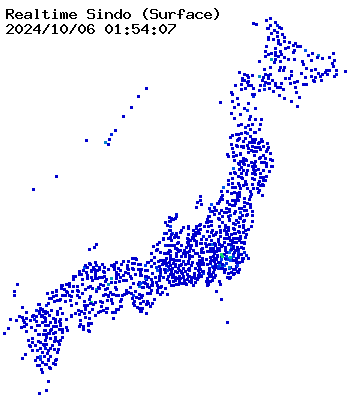
\includegraphics[width=0.5\linewidth]{sample-kmoni.png}
    \caption{Sample GIF image achieved from 'Kyoshin' Monitor}
    \label{fig:sample-kmoni}
\end{figure}

\subsubsection{Extracting colour for each observation point}

Unfortunately, it seems to the author (and is widely accepted in the EEW monitoring app development society) that the position of the points (squares) on the image does not follow any significant pattern of position, i.e. there is no obvious conversion of coordinates to us from the official longitude/latitude locations to the positions on the image. Therefore, a manual conversion one-to-one mapping has to be developed.

NIED does have an official released list of observation points, which include their names and positions. This list has around 1700 of those observation points. However, in the actual image (like those in Figure \ref{fig:sample-kmoni}), there are only 1000 of those in use in real time, consistent with K-NET's official introduction, and the rest 700 of those are invalid observation points. Therefore, it will be worth removing them from the list of earthquake monitoring points, before attempting to make the dictionary.

Unfortunately, 1000 is still quite a lot for us to deal with. Luckily, Ingen who used a similar approach to develop the KEVI application has already made such a mapping inside his open-source application in the file \href{https://github.com/ingen084/KyoshinEewViewerIngen/blob/develop/src/KyoshinEewViewer/Assets/ShindoObsPoints.mpk.lz4}{ShindoObsPoints.mpk.lz4} within \GitHubHref{ingen084}{KyoshinEewViewerIngen}, and even developed an editor for this at \GitHubHref{ingen084}{KyoshinShindoPlaceEditor}.

Due to the limited time for this NEA, the author will primarily use the pre-determined observation points for the K-NET and the KiK-net by Ingen in JSON format.

This paragraph referred to \autocite{blog-ingen-kmoni-data}.

\subsubsection{Converting colour to number format for further processing}

The true numerical data does not seem fully necessary at the first glance (since we might just as well just achieve the colour from the image and just plot them on the map, without the need to convert to a colour and back). However, for us to detect the shake in certain regions, it is necessary for us to achieve the numerical value to run the algorithm on it. Nevertheless, it is just good to have the number for us to have the numerical value for potential future developments.

\begin{figure}[htp]
    \centering
    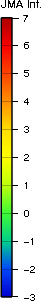
\includegraphics[scale = 0.6]{jma-scale.png}
    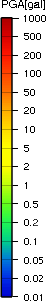
\includegraphics[scale = 0.6]{pga-scale.png}
    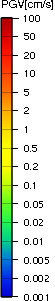
\includegraphics[scale = 0.6]{pgv-scale.png}
    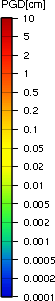
\includegraphics[scale = 0.6]{pgd-scale.png}
    \caption{Scale colours of different measurements}
    \label{fig:scale-colour}
\end{figure}

As shown in Figure \ref{fig:scale-colour}, the NIED 'Kyoshin' Monitor does indeed provide a scale of colours and reference to numerical values. However, there is a chance that a certain colour is not 'exactly' mapped on the scale, and further concerning that it is very slow and difficult to 'loop over' a colour legend, it is necessary to have an algorithmic-approach (numerical mapping-based approach) to map the colours in the colour space to numerical values (and back) is necessary.

\paragraph{Abstraction of colour scale}

Notice that the scale for PGA/PGV/PGD follow a logarithmic scale, while measured intensity follows a linear scale (though noting that the way intensity and magnitude is calculated is logarithmic as well). Therefore, if we normalise the vertical distance from the bottom of the axis \(h\) to \(0 \leq h \leq 1\) (i.e. \(h = 0\) at the bottom of the scale, \(h = 1\) at the top of the scale), and if we denote intensity using \(I\) in JMA scale, PGA as \(a\) in gal, PGV as \(v\) in cm per second, and PGD as \(s\) in cm, from the scale, the following transforming formulae obviously hold:
\begin{align*}
    I  = 10h - 3     & \iff h      = \frac{I + 3}{10}, \\
    a  = 10^{5h - 2} & \iff h  = \frac{\lg a + 2}{5},  \\
    v  = 10^{5h - 3} & \iff h  = \frac{\lg v + 3}{5},  \\
    x  = 10^{5h - 4} & \iff h  = \frac{\lg x + 4}{5}.  \\
\end{align*}

However, it is worth noting that NIED did use \(1, 2, 5, 10\) on the logarithmic scale at equal intervals, so it is not a perfect logarithmic scale. The author is unsure why they designed the scale like this, nor if it's an intended approximation. Nevertheless, the logarithmic scale is a good enough approximation.

The next step is to develop a mapping from this colour space \(\mathcal{C}\) to \(h\), which of course should be invertible. Denote this as \(f: [0, 1] \to \mathcal{C}\).

\paragraph{Describing colour numerically}

We consider using a suitable base to decompose \(\mathcal{C}\). The colour of the given scale is an immediate suggestion to use a base containing \textbf{hue}, which in fact is designed to describe how human perceive colour, and unlike RGB and CMYK which uses principle colours to describe colour. A hue scale is shown in Figure \ref{fig:hue-scale}.

\begin{figure}[htp]
    \centering
    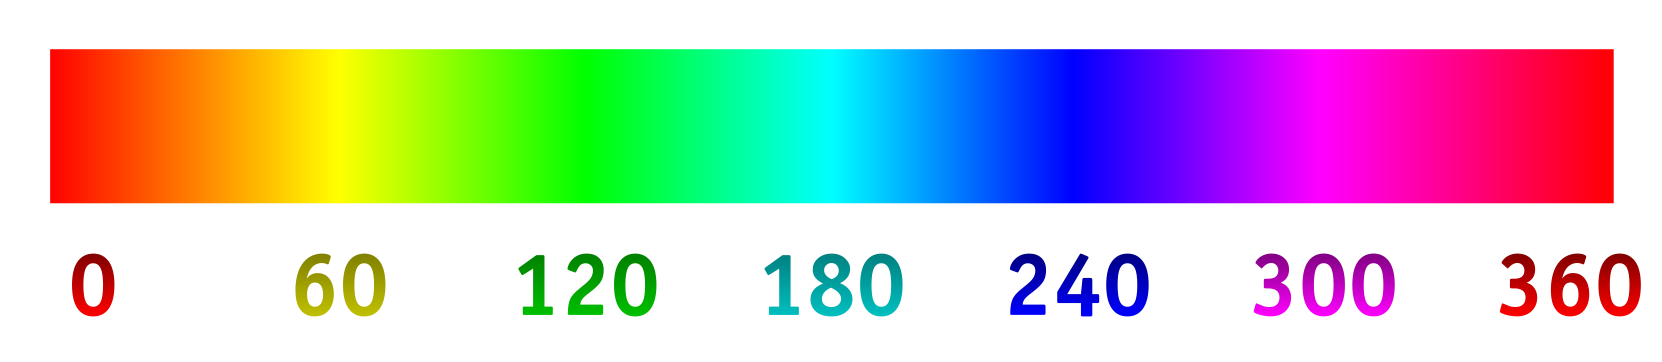
\includegraphics[scale = 0.15]{hue-scale.png}
    \caption{The hue scale in HSL/HSV encoding}
    \label{fig:hue-scale}
\end{figure}

Therefore, a colour in the colour space \(\mathcal{C}\) can be represented as a 3-D vector \(\mathcal{C} \ni C = (H, S, V)\), where \(H \in [0, 360)\) in degrees is the hue value, \(S \in [0, 1]\) stands for the saturation, and \(V \in [0, 1]\) stands for the value (a brightness). And hence we will be able to decompose \(f\) into three components \(f = \left(f_H, f_S, f_V\right)\).

Figure \ref{fig:hsv-against-row} plots the values of \(H, S\) and \(V\) against \(h\) (this is the graph of \(f\) and its components) of discrete values of \(h\), and depending on the result we will attempt some fit/regression to a suitable function.

\begin{figure}[htp]
    \centering
    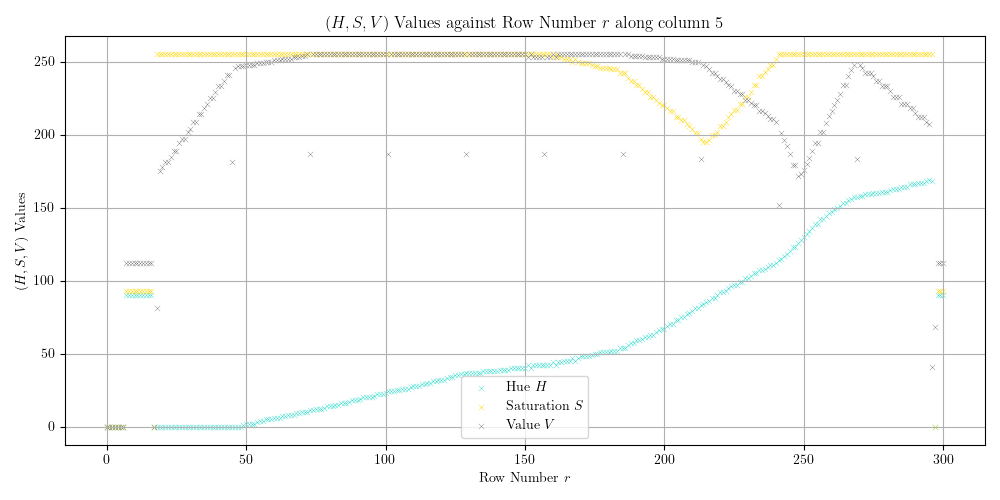
\includegraphics[scale = 0.60]{hsv-against-row.png}
    \caption{The values of \((H, S, V)\) against pixel row \(r\)}
    \label{fig:hsv-against-row}
\end{figure}

Notice that in this plot, all values of \((H, S, V)\) in fact range from \(0\) to \(255\), as in an 8-bit binary.

It is worth noting that the scale has some space on the top (to show the type), and some space at the bottom. Notice that when the row \(r = 17\) and \(r = 297\) have values significantly different, so we extract the rows \(r = 18\) and \(r = 296\) to correspond (linearly) to \(h = 1\) and \(h = 0\), i.e.,
\[
    h = 1 - \frac{r - 18}{278}.
\]

Figure \ref{fig:hsv-against-h} shows the result of this transformation being applied.

\begin{figure}[htp]
    \centering
    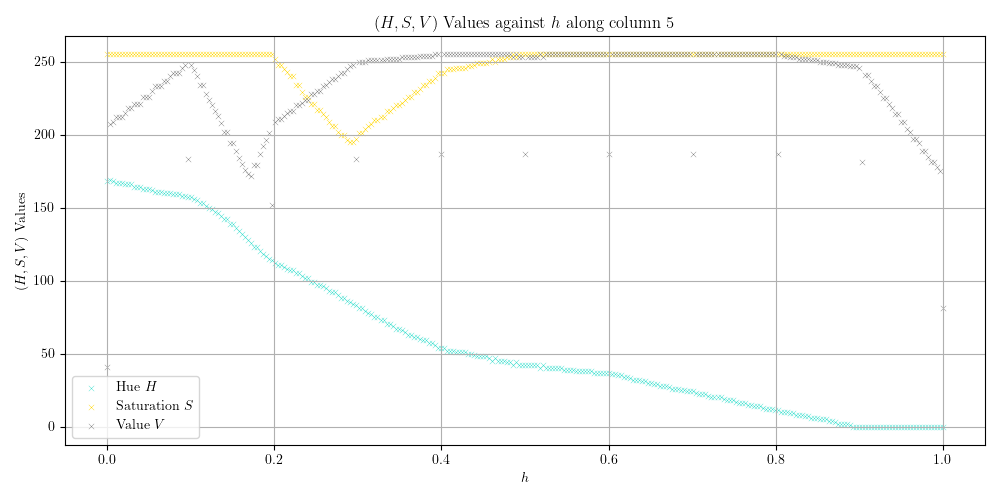
\includegraphics[scale = 0.60]{hsv-against-h.png}
    \caption{The values of \((H, S, V)\) against normalised height \(h\)}
    \label{fig:hsv-against-h}
\end{figure}

From here onwards, all values of \((H, S, V)\) will be adjusted to be within the range which they should be in, i.e. \(H \in [0, 360), S \in [0, 1], V \in [0, 1]\).

\paragraph{Finding \(f_H\) in terms of \(h\)}

We consider finding \(f_H\) first, which is the cyan line. Notice that its trend can be split into 4 parts:
\begin{itemize}
    \item \(h \in [0, 0.1]\): linear;
    \item \(h \in [0.1, 0.6]\): curving, ideally a cubic;
    \item \(h \in [0.6, 0.9]\): linear;
    \item \(h \in [0.9, 1]\): constant (0).
\end{itemize}

\begin{table}[htp]
    \centering

    \begin{tabular}{|c|c|}
        \hline
        \(h\) & \(H = f_H(h)\) \\
        \hline
        0     & 237            \\
        0.1   & 222            \\
        0.6   & 51             \\
        0.9   & 0              \\
        1     & 0              \\
        \hline
    \end{tabular}
    \caption{Initial values for \(f_H\)}
    \label{tab:h-against-h-iv}
\end{table}

Furthermore, boundary conditions in Table \ref{tab:h-against-h-iv} are applied to ensure that the function is continuous and nicely-behaving while matching the existing data. We use the following function to apply the fit:
\[
    f_H(h) = \begin{cases}
        -150h + 237, & h \in [0, 0.1],   \\
        \odot,       & h \in [0.1, 0.6], \\
        -170h + 153, & h \in [0.6, 0.9], \\
        0,           & h \in [0.9, 1].
    \end{cases}
\]

Here,
\begin{align*}
    \odot & = \frac{222 \cdot (h - 0.3) \cdot (h - 0.4) \cdot (h - 0.6)}{(0.1 - 0.3) \cdot (0.1 - 0.4) \cdot (0.1 - 0.6)} \\
          & + \frac{y_1 \cdot (h - 0.1) \cdot (h - 0.4) \cdot (h - 0.6)}{(0.3 - 0.1) \cdot (0.3 - 0.4) \cdot (0.3 - 0.6)} \\
          & + \frac{y_2 \cdot (h - 0.1) \cdot (h - 0.3) \cdot (h - 0.6)}{(0.4 - 0.1) \cdot (0.4 - 0.3) \cdot (0.4 - 0.6)} \\
          & + \frac{51 \cdot (h - 0.1) \cdot (h - 0.3) \cdot (h - 0.4)}{(0.6 - 0.1) \cdot (0.6 - 0.3) \cdot (0.6 - 0.4)}.
\end{align*}

Here, \(m_1\) is the gradient of the line for \(h \in [0, 0.1]\), \(y_1 = f_H(0.3), y_2 = f_H(0.4)\) for \(h \in [0.1, 0.6]\) (using Lagrange Polynomial), and the equation between \(h \in [0.6, 0.9]\) is in fact fixed due to the initial conditions.

By applying a curve fit to the original data, the following results are obtained:
\[
    (y_1, y_2) = (115, 79.5).
\]

Plotting \(H\) and \(f_H(h)\) against \(h\) gives us Figure \ref{fig:h-against-h}, which is decent.

\begin{figure}[htp]
    \centering
    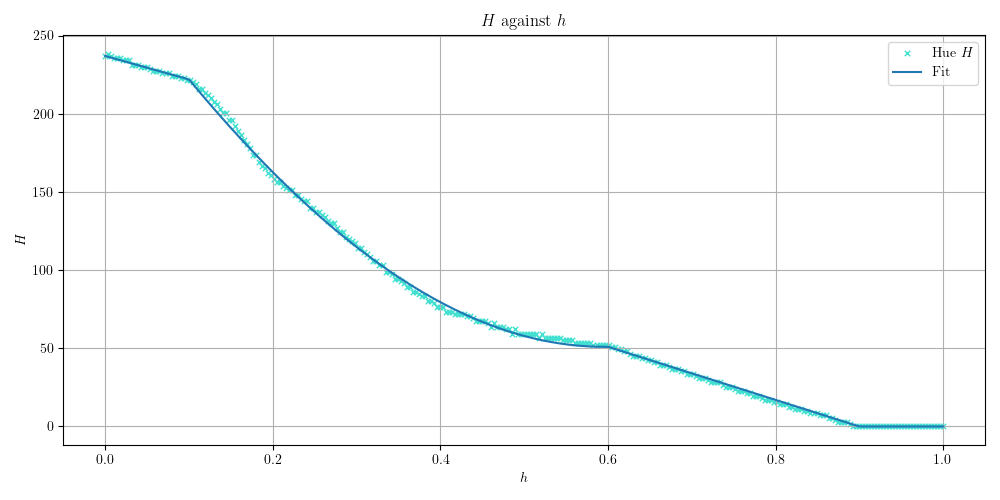
\includegraphics[scale = 0.60]{h-against-h.png}
    \caption{The fit result for \(f_H: h \mapsto H\)}
    \label{fig:h-against-h}
\end{figure}

\paragraph{Finding \(f_S\) in terms of \(h\)}

As for \(f_S(h)\), the obvious thing to do is to split it into 5 (4) piecewise functions, specifically \(f_S = 1\) for \(h \in [0, 0.2] \cup [0.5, 1]\), and three linear functions for \(h \in [0.2, 0.29], h \in [0.29, 0.4]\) and \(h \in [0.4, 0.5]\). Initial values are included in Table \ref{tab:s-against-h-iv}.

\begin{table}[htp]
    \centering

    \begin{tabular}{|c|c|}
        \hline
        \(h\) & \(S = f_S(h)\) \\
        \hline
        0     & 1              \\
        0.2   & 1              \\
        0.29  & 0.765          \\
        0.4   & 0.95           \\
        0.5   & 1              \\
        1     & 1              \\
        \hline
    \end{tabular}
    \caption{Initial values for \(f_S\)}
    \label{tab:s-against-h-iv}
\end{table}

This gives us that
\[
    f_S(h) = \begin{cases}
        1,              & h \in [0, 0.2],    \\
        -2.611h + 1.522 & h \in [0.2, 0.29], \\
        1.682h + 0.277, & h \in [0.29, 0.4], \\
        0.5h + 0.75     & h \in [0.4, 0.5],  \\
        1,              & h \in [0.5, 1].
    \end{cases}
\]

Plotting this out gives Figure \ref{fig:s-against-h}.

\begin{figure}[htp]
    \centering
    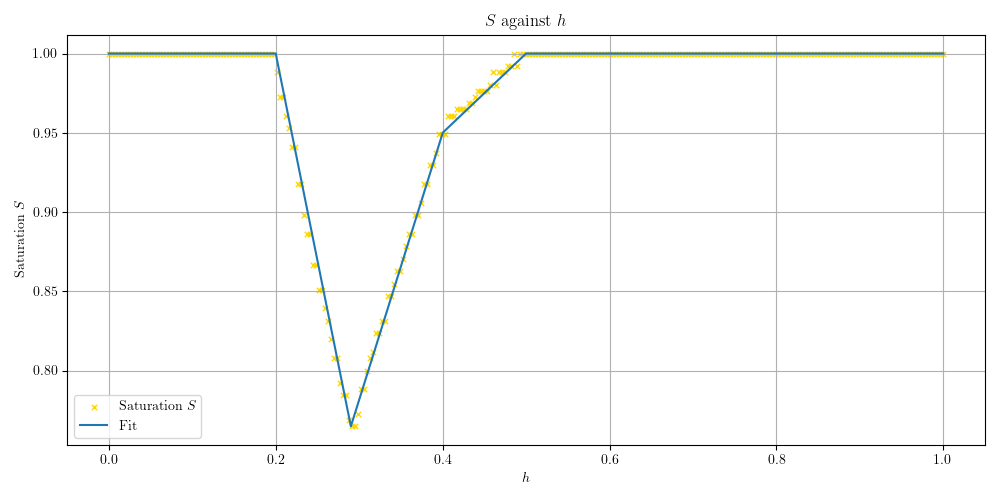
\includegraphics[scale = 0.60]{s-against-h.png}
    \caption{The fit result for \(f_S: h \mapsto S\)}
    \label{fig:s-against-h}
\end{figure}

\paragraph{Finding \(f_V\) in terms of \(h\)}

As for \(f_V(h)\), we shall divide it into even more piecewise linear functions. Specifically, I chose to divide the interval \([0, 1]\) at \(0.1, 0.172, 0.2, 0.3, 0.4, 0.8\) and \(0.9\). Initial values are included in Table \ref{tab:v-against-h-iv}.

\begin{table}[htp]
    \centering

    \begin{tabular}{|c|c|}
        \hline
        \(h\) & \(V = f_V(h)\) \\
        \hline
        0     & 0.8            \\
        0.1   & 0.98           \\
        0.172 & 0.66           \\
        0.2   & 0.82           \\
        0.3   & 0.98           \\
        0.4   & 1              \\
        0.8   & 1              \\
        0.9   & 0.97           \\
        1     & 0.68           \\
        \hline
    \end{tabular}
    \caption{Initial values for \(f_V\)}
    \label{tab:v-against-h-iv}
\end{table}

This gives us the piecewise function
\[
    f_V(h) = \begin{cases}
        1.8h + 0.8,      & h \in [0, 0.1],     \\
        -4.444h + 1.424, & h \in [0.1, 0.172], \\
        5.714h - 0.323,  & h \in [0.172, 0.2], \\
        1.6h + 0.5,      & h \in [0.2, 0.3],   \\
        0.2h + 0.92,     & h \in [0.3, 0.4],   \\
        1,               & h \in [0.4, 0.8],   \\
        -0.3h + 1.24,    & h \in [0.8, 0.9],   \\
        -2.9h + 3.58,    & h \in [0.9, 1].
    \end{cases}
\]

Plotting this out gives us Figure \ref{fig:v-against-h}.

\begin{figure}[htp]
    \centering
    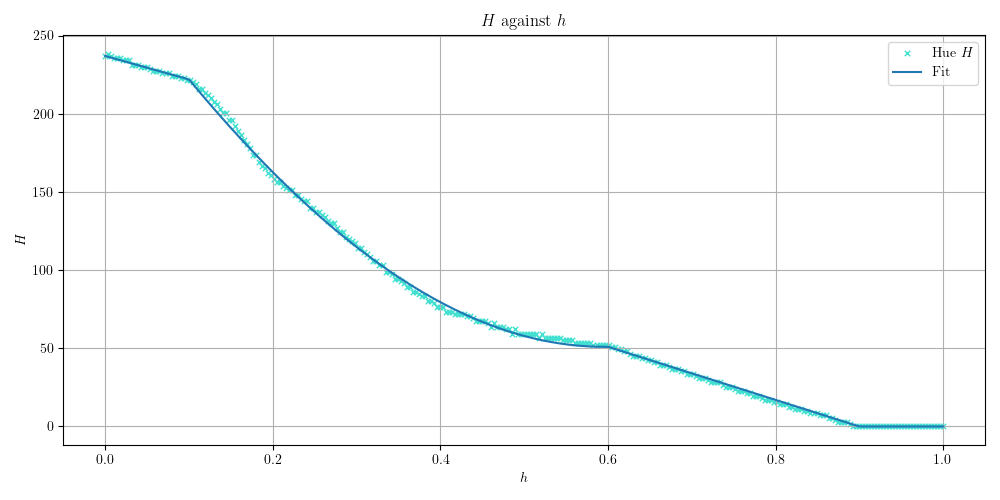
\includegraphics[scale = 0.60]{v-against-h.png}
    \caption{The fit result for \(f_V: h \mapsto V\)}
    \label{fig:v-against-h}
\end{figure}

Note that in this plot, \(V\) when \(h = 0\) or \(h = 1\) is excluded, since just like every \(h = 0.1 k\) for some \(k \in \mathbb{N}\), they are anomalies created by the horizontal black line in the scale.

\paragraph{Finding \(f^{-1}\)}

To find \(f^{-1}: \mathcal{C} \to [0, 1]\), we do not need necessarily to find an expression of \(h\) in terms of \((H, V, S)\). If we notice that \(f_H\) is one-to-one on \(h \in [0, 0.9]\), and \(f_V\) is one-to-one on \(h \in [0.9, 1]\), we can use \(f_H^{-1}\) to determine \(h\) from \(H\) only if \(H\) is non-zero, and use \(f_V^{-1}\) otherwise.

\[
    f^{-1}(H, S, V) = \begin{cases}
        f_H^{-1}(H), & H \neq 0, \\
        f_V^{-1}(V), & H = 0.
    \end{cases}
\]

Notice that for \(h \in [0.1, 0.6]\), \(f_H\) is a cubic and is not easily invertible. However, it would be plausible to use a binary-search algorithm to find \(h\) based on \(H\) since it is monotonic, and it is within a reasonable amount of time, to relatively good precision. Otherwise, on the linear parts, it is fine to simply mathematically invert it.

Algorithm \ref{alg:cap} describes the logic. Note that, this algorithm uses different \(V\) ranges from before (which is consistent with SkiaSharp library in C\#), and the ranges is \(V \in [0, 100]\). Notice that, \(\epsilon(h)n\) and \(\epsilon(H)\) are two constant values that determines the precision of such binary search, and they are chosen to be \(0.01\) and \(0.5\) in the implementation.

\begin{algorithm}[htp]
    \caption{Algorithm for \(f^{-1}\)}\label{alg:cap}
    \begin{algorithmic}
        \Require \(H \in [0, 360)\)
        \Require \(S \in [0, 100]\)
        \Require \(V \in [0, 100]\)
        \Ensure \(h \in [0, 1]\)
        \State \(V \gets V / 100\) \Comment{Normalise \(V\)}
        \If{\(V\) is \(0\)} \Comment{Use \(V\)}
        \State \Return \((V - 3.50) / (-2.9)\)
        \Else \Comment{Use \(H\)}
        \LComment{Deal with out-of-range \(H\)s, and use inverse linear functions}
        \If{\(H \geq 222\)}
        \State \Return \((H - 237) / (-150)\)
        \ElsIf{\(H \leq 51\)}
        \State \Return \((H - 153) / (-170)\)
        \LComment{Inverse-Cubic by Binary Search, with set errors}
        \Else
        \State \(l \gets 0.1\)
        \State \(r \gets 0.6\)
        \LComment{Checks if the normalised height is already precise enough}
        \While{\(r - l \geq \epsilon(h)\)}
        \State \(m \gets (l + r) / 2\)
        \State \(c \gets \Call{Height to Hue}{m}\)
        \LComment{Checks if the calculated hue is already precise enough}
        \If{\(\left\lvert c - H\right\rvert \leq \epsilon(H)\)}
        \State \Return \(m\)
        \ElsIf{\(c > H\)}
        \State \(l \gets m\)
        \ElsIf{\(c < H\)}
        \State \(r \gets m\)
        \EndIf
        \EndWhile

        \State \Return \((l + r) / 2\)
        \EndIf
        \EndIf
    \end{algorithmic}
\end{algorithm}

\subsubsection{Flowchart of data and sidenotes}

To summarise, we discussed the mapping from the colour space\(\mathcal{C}\) to the normalised height \(h\), and back, and we also discussed how \(h\) is related with the measured intensity \(I\), the PGA \(a\), the PGV \(v\), and the PGD \(x\). They can be transformed forwards and backwards using simple mathematical explicit relations, and specifically for \(f_H^{-1}(H)\) will use a binary search algorithm.

Figure \ref{fig:kmoni-data-flow} shows the data flow, Figure \ref{fig:variable-relation} shows the relation between abstract variables, and \ref{fig:generated-colour} shows the result of colour generated compared with the original.

\begin{figure}[htp]
    \centering
    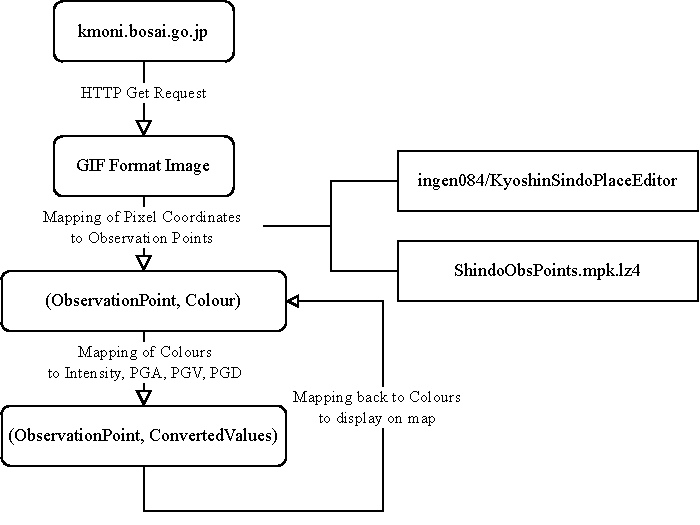
\includegraphics[width=0.8\linewidth]{kmoni-data-flow.pdf}
    \caption{Flow of data in NIED data sources}
    \label{fig:kmoni-data-flow}
\end{figure}

\begin{figure}[htp]
    \centering
    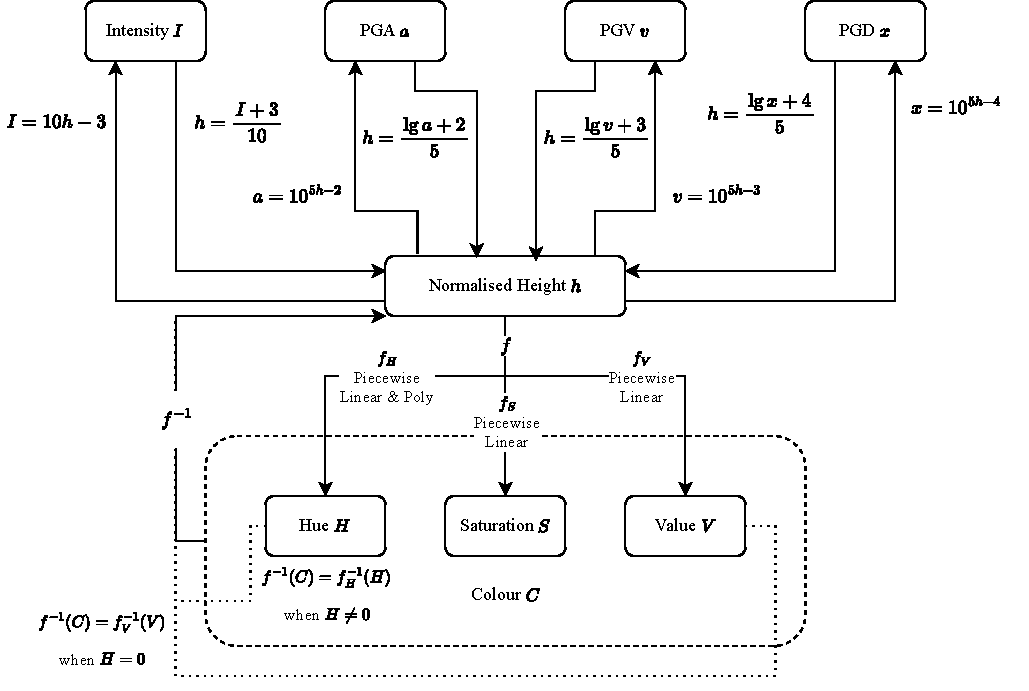
\includegraphics[width=0.9\linewidth]{variable-relation.pdf}
    \caption{Relation between abstract variables}
    \label{fig:variable-relation}
\end{figure}

\begin{figure}[htp]
    \centering
    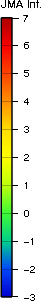
\includegraphics[scale = 0.6]{jma-scale.png}
    
\includegraphics[scale = 0.6]{generated-colour.png}
    \caption{Colour generated using fitted functions}
    \label{fig:generated-colour}
\end{figure}

It is worth noting that an existing NuGet Library, \GitHubHref{ingen084}{KyoshinMonitorLib} and introduced in \autocite{blog-ingen-kmoni-nuget-lib} which is designated to manage intensities, as well as extracting intensities from the 'Kyoshin' monitor. This NEA did refer to this for some guidance but is not dependent on this library, and its necessary functionalities within the scope of this NEA is realised again using the author's own code. The developer of this library did also mention that it is quite purpose-built so might not be suitable for general use.

It is also worth noting that, technically, scraping the data from the 'Kyoshin' monitor page of NIED is not explicitly allowed, but not explicitly banned either. However, extracting and displaying numerical data in the application is strictly banned by the NIED, and therefore the numerical values will only serve as internal values of the application and will not be displayed to the users in any way.

This paragraph referred to \autocite{blog-jquake-poly-fit}. The code used for this section is in Listing \ref{code:poly-fit}.

\subsection{DM-D.S.S. Data Source}

DM-D.S.S. is a well-structured official data source with low latency and reliable information and services. This is going to be the primary data source for most part of the application.

Their APIs are split into two types: HTTP based requests and WebSocket based connections. HTTP based requests are typically for more static information, while WebSocket connections are for live time-essential data feeds, such as the EEW warnings, tsunami warnings and latest earthquake information.

\subsubsection{Authorisation}

There are two types of authorisation that DM-D.S.S. supports, API Keys and OAuth2 Access Tokens.

API Keys access tokens are extremely easy to program, since it simply uses Basic Authorisation in the header, and uses the key as the username (without a password). It uses the Basic BasicBase64 Authorisation encoding. However, this introduces an extra layer of complexity for the users, since they would have to go to the settings of the DM-D.S.S. webpage and achieve an API Key to paste into the application, as shown in Figure \ref{fig:api-key-control-panel}.

\begin{figure}[htp]
    \centering
    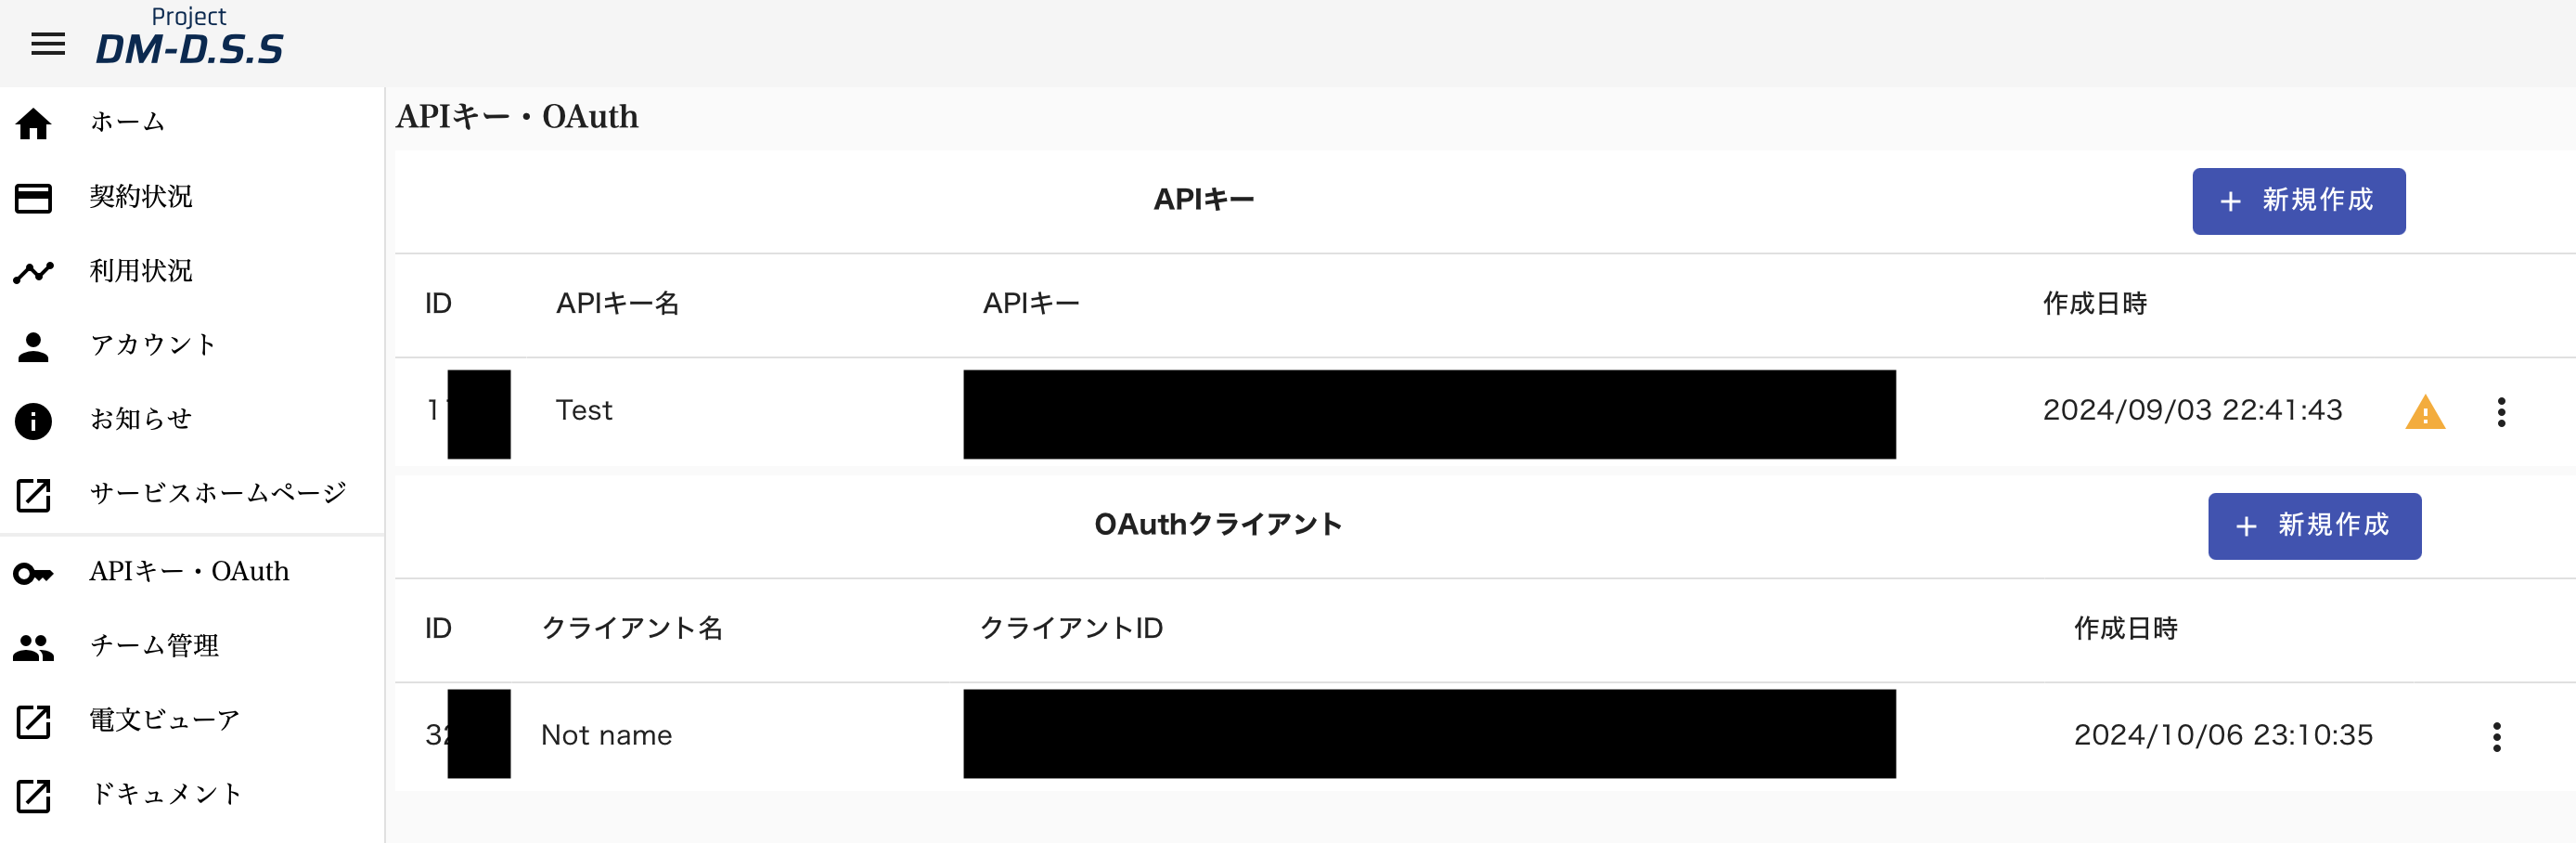
\includegraphics[width=0.7\linewidth]{api-key-control-panel.png}
    \caption{Control panel for API Keys}
    \label{fig:api-key-control-panel}
\end{figure}

As for OAuth2, it will be much simpler for the users, since it will provide the user with a login interface on the website, and ask them to give the program certain permissions, which is just a few simple clicks. Rather than using the user as a bridge for sharing the credentials with the application, they are shared between the authorisation server (DM-D.S.S.) and the application directly, without the need for the user to deal with such human-unreadable codes.

\paragraph{OAuth 2.0}

OAuth 2.0 is a standard protocol that allows a user to authorise an application without sharing any of their credentials. Figure \ref{fig:oauth-outline} gives a brief outline of the procedure involved.

\begin{figure}[htp]
    \centering
    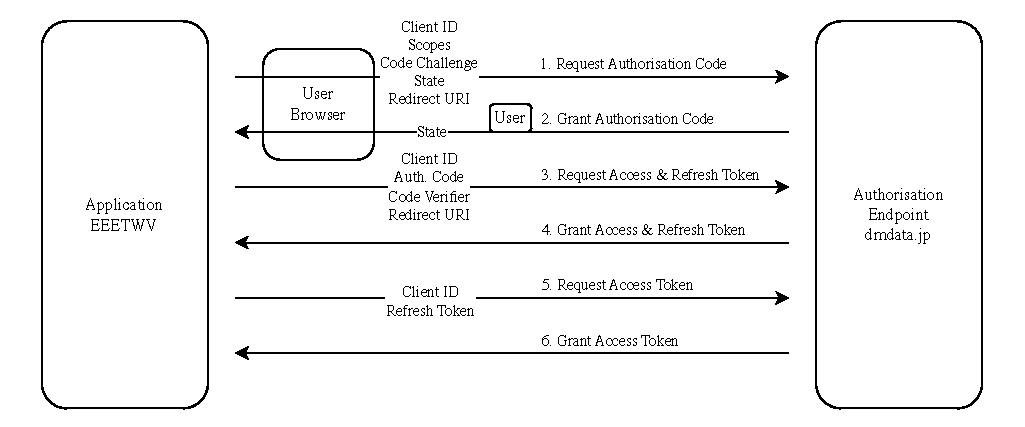
\includegraphics[width=\linewidth]{oauth-outline.pdf}
    \caption{OAuth Procedure Outline}
    \label{fig:oauth-outline}
\end{figure}

\subparagraph{Authorisation Code}

The authorisation begins with the application requesting an \textbf{authorisation token} from the authorisation endpoint, via the user's browser. This is the only step where the user has to be involved, but all they have to do is log-in to their DM-D.S.S. account and click the 'grant' button on the page.

First, the user launches the browser to the authorisation endpoint (Step 1)
\begin{center}
    \url{https://manager.dmdata.jp/account/oauth2/v1/auth}
\end{center}
with the following parameters:
\begin{itemize}
    \item \Code{client_id}: the client ID for the application to grant (which is public and safe to be seen by the user);
    \item \Code{redirect_uri}: redirect URL for the endpoint to redirect to, to inform the application of the authorisation results;
    \item \Code{response_type}: \Code{code}
    \item \Code{response_mode}: the way to response to the application (we will only use the response type \Code{query});
    \item \Code{scope}: the string containing the permissions the application is requesting, separated by a space;
    \item \Code{state}: the state which will be returned by the return query to prevent CSRF attacks;
    \item \Code{code_challenge}: the code challenge for PKCE;
    \item \Code{code_challenge_method}: the way to encode the code challenge (we will use \Code{S256}).
\end{itemize}

At the same time as launching the browser, the program should start a listener on the local IP address and port specified in the redirect URL, and wait until it receives a request from the browser. In the response (Step 2), it will contain two parameters: \Code{code} which contains the authorisation code (which is only valid for 10 minutes), and \Code{state} which should be the same as the state sent in the request.

The reason why the \textbf{state} is essential is to prevent CSRF (Cross-Site Request Forgery) attacks, where the application can make sure the response is truly corresponding to the request the application made (not by any other applications), and no one forged a response to the application (pretended to be the browser acting as authorisation endpoint). Verifying the state is essential for the security of the application.

If the request fails, the return query will return the \Code{error}, and with the \Code{state} as well. Table \ref{tab:oauth2-auth-code-errors} includes a table of errors that could occur in the authorisation code request.

\begin{table}
    \centering
    \begin{tabular}{cc}
        Error Code                               & Description                                            \\
        \hline
        \Code{invalid_request}                   & The parameters are invalid.                            \\
        \Code{invalid_client}                    & The Client ID is invalid.                              \\
        \Code{invalid_redirect_url}              & The redirect URL is not supported by the Client ID.    \\
        \Code{invalid_scope}                     & The scope string is invalid.                           \\
        \Code{unauthorized_client}               & The client to authorise using this method is invalid.  \\
        \Code{access_denied}                     & The access is denied.                                  \\
        \Code{recaptcha_verification_failed}     & The reCAPTCHA verification failed.                     \\
        \Code{unsupported_response_type}         & The response type is not recognised.                   \\
        \Code{unsupported_code_challenge_method} & The code challenge method is not recognised.           \\
        \Code{no_signin}                         & The user is not signed in (usually should not happen). \\
        \Code{server_error}                      & The internal server encountered an error.
    \end{tabular}
    \caption{Error codes for authorisation code step in OAuth2}
    \label{tab:oauth2-auth-code-errors}
\end{table}

In the application, only the errors \Code{access_denied}, \Code{recaptcha_verification_failed}, \Code{no_signin} and \Code{server_error} should appear (and the final two shouldn't appear usually), since all other errors are due to issue with design of the application.

\subparagraph{Refresh and Access Token}

After this step, the program will use the authorisation token to request an \textbf{access token} which comes with a \textbf{request token} (Step 3). The program will send an HTTP POST request to the token endpoint
\begin{center}
    \url{https://manager.dmdata.jp/account/oauth2/v1/token}
\end{center}
with the following query parameters, in URL Encoded form:
\begin{itemize}
    \item \Code{client_id}: the client ID for the application to grant (which is public and safe to be seen by the user);
    \item \Code{grant_type}: \Code{authorization_code};
    \item \Code{code}: the authorisation code received from the previous step;
    \item \Code{redirect_uri}: the redirect URL used in the previous step;
    \item \Code{code_verifier}: the original version of the code challenge used in the previous step.
\end{itemize}

Now the reason of the code challenge and code verifier is apparent (they are part of PKCE, Proof Key for Code Exchange): since the code challenge is a hashed version of the code verifier and is exchanged in the first step, the code verifier (the plain version) is used to prove that the application is the same as the one that requested the authorisation code. This means, if a man-in-the-middle acquired the authorisation code and the code challenge, they would not be able to use it, since it requires them to reverse hash the code challenge to get the code verifier, which is impossible in a reasonable amount of time. To ensure the security, the code verifier should be generated randomly and be very long, and disposed after each use.

The response (Step 4) will be JSON format, as shown in Listing \ref{code:oauth-access-token-request}.

\begin{listing}[htp]
    \inputminted{json}{code/OAuthAccessTokenRequest.json}
    \caption{Response for OAuth Access Token Request}
    \label{code:oauth-access-token-request}
\end{listing}

The properties \Code{token_type}, and \Code{expires_in} are constants, the \Code{scope} are the scopes which are authorised for, and the most important two are the \Code{access_token} and \Code{refresh_token}.

The refresh token is a long-living token, and it has lifetime 183 days in DM-D.S.S., resetting every time a new access token is acquired (see below). On the other hand, the access token is a short-living token, and it has lifetime 6 hours only. This does not mean that the access token should be disposed per-use -- it should be reused within the application, and only when it expires, a new access token should be requested using the refresh token. However, when the application is closed, only the refresh token should be stored, and the access token revoked -- next time the application launches, the access token should be acquired again.

If the request failed, then an error will be returned, also in JSON format, as shown in Listing \ref{code:oauth-error}.

\begin{listing}[htp]
    \inputminted{json}{code/OAuthError.json}
    \caption{Error for OAuth Access Token Request}
    \label{code:oauth-error}
\end{listing}

Table \ref{tab:oauth2-access-token-errors} includes a table of errors that could occur in the authorisation code request.

\begin{table}
    \centering
    \begin{tabular}{cc}
        Error Code                    & Description                                           \\
        \hline
        \Code{invalid_request}        & The parameters are invalid.                           \\
        \Code{invalid_client}         & The Client ID is invalid.                             \\
        \Code{invalid_redirect_url}   & The redirect URL is not supported by the Client ID.   \\
        \Code{invalid_grant}          & The authorisation code is invalid.                    \\
        \Code{invalid_code_verifier}  & The PKCE verification failed.                         \\
        \Code{unauthorized_client}    & The client to authorise using this method is invalid. \\
        \Code{unsupported_grant_type} & The grant type is not recognised.                     \\
        \Code{server_error}           & The internal server encountered an error.
    \end{tabular}
    \caption{Error codes for access token step in OAuth2}
    \label{tab:oauth2-access-token-errors}
\end{table}

The only error that should occur here is \Code{server_error}.

\subparagraph{Refreshing Access Token}

Finally, Step 5 and 6 will be repeated multiple times in the application, to request a new access token using the provided refresh token. Similarly, the request will be a post request, but only requiring the \Code{client_id}, the \Code{grant_type} (as \Code{refresh_token}) and \Code{refresh_token} in the URL Encoded form, to the same endpoint.

The response JSON will be exactly the same, except the refresh token is not included again. It includes the newly acquired access token. In case of an error, all errors in Table \ref{tab:oauth2-access-token-errors} apart from \Code{invalid_redirect_url} and \Code{invalid_code_verifier} could occur. In this case however, there could be a chance of \Code{invalid_grant}, if the application is closed for a very long period of time and the refresh token expired. In this case, the user should be asked to re-authorise the application.

\subparagraph{Revoking Tokens}

Tokens should be revoked whenever they are no longer used. The revoke is done by sending a POST request to the revoke endpoint, which is
\begin{center}
    \url{https://manager.dmdata.jp/account/oauth2/v1/revoke},
\end{center}
with the following parameters:
\begin{itemize}
    \item \Code{client_id}, the client ID;
    \item \Code{token}, the token to be revoked.
\end{itemize}

The API will not return anything if successful, and if the token is already invalid, it will still be successful.

An error will be similar to that in Table \ref{tab:oauth2-access-token-errors}, but only \Code{invalid_request}, \Code{invalid_client} and \Code{server_error} could occur. Nonetheless, only \Code{server_error} should occur in the application.

\subparagraph{Flowchart}

In terms of the design of classes to support OAuth 2.0, there should be two separate classes responsible for this: one for acquiring the authorisation code and the refresh token, and the other for acquiring the access token using the refresh token.

Figure \ref{fig:oauth-flowchart-authorisation-refresh} shows the flowchart for the former, and \ref{fig:oauth-flowchart-access-check} shows the flowchart for the latter.

\begin{figure}[htp]
    \centering
    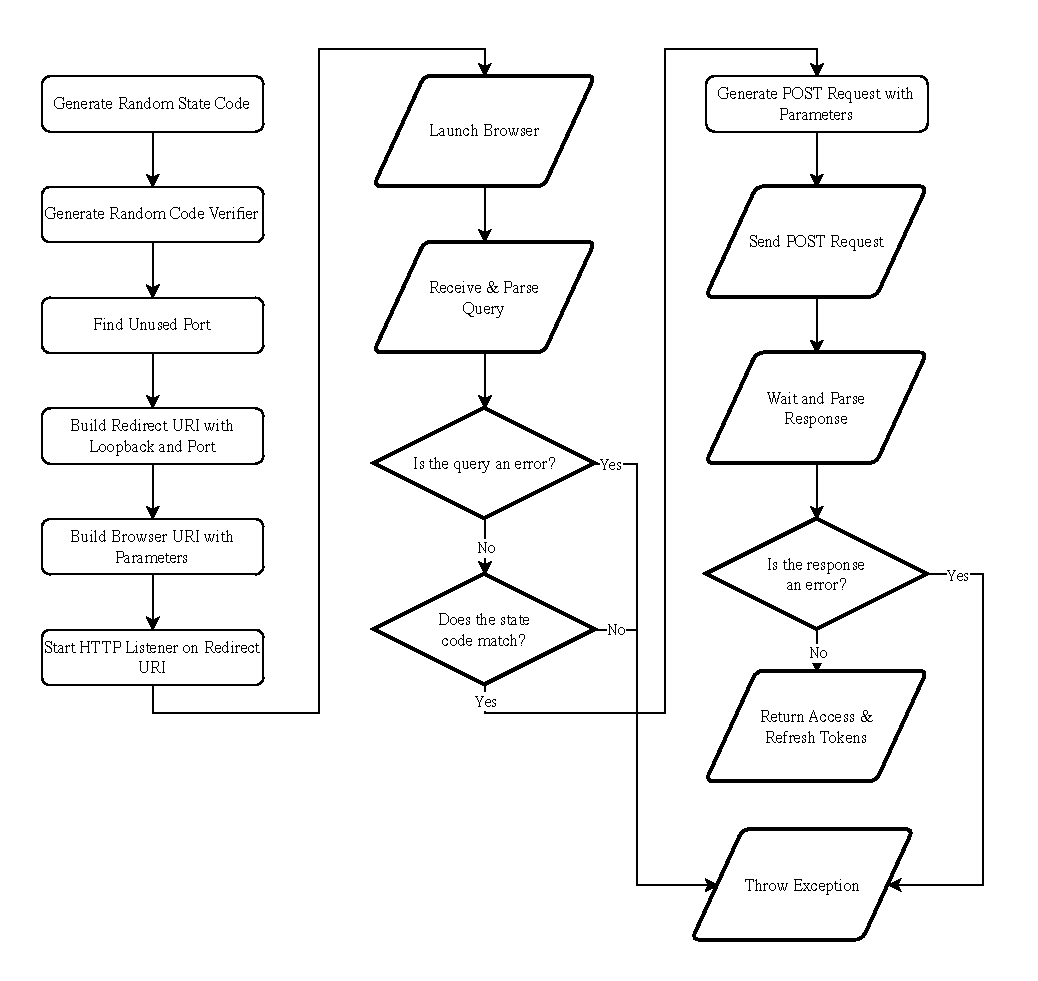
\includegraphics[width=\linewidth]{oauth-flowchart-authorisation-refresh.pdf}
    \caption{Flowchart for OAuth 2.0 Authorisation Code and New Refresh Token}
    \label{fig:oauth-flowchart-authorisation-refresh}
\end{figure}

\begin{figure}[htp]
    \centering
    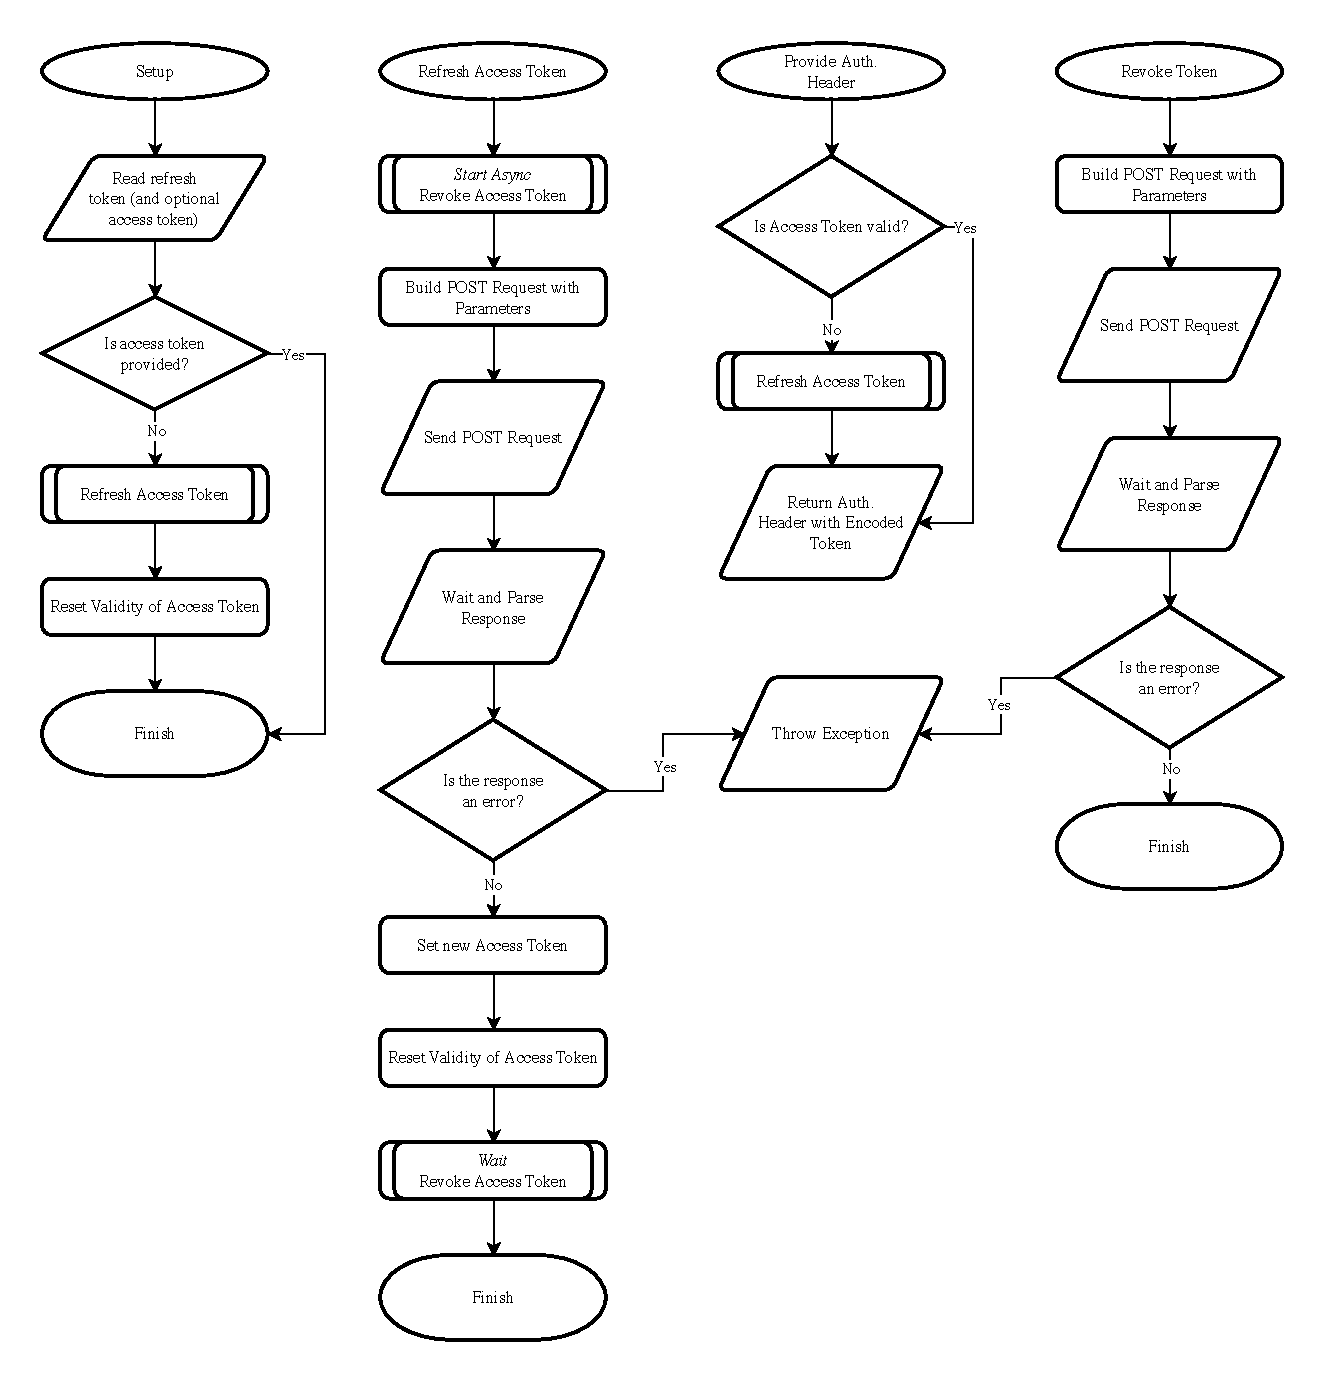
\includegraphics[width=\linewidth]{oauth-flowchart-access-check.pdf}
    \caption{Flowchart for OAuth 2.0 Acquire Access Token using Refresh Token}
    \label{fig:oauth-flowchart-access-check}
\end{figure}

Figure \ref{fig:oauth-flowchart-access-check} represents the behaviour of the OAuth2 main class for authentication, while the previous figure \ref{fig:oauth-flowchart-authorisation-refresh} represents the behaviour of the helper.

\subparagraph{Notes}

For the purposes of this NEA, we will primarily use the API Key to test the application for accessing  way of accessing DM-D.S.S. since it will be easier to code and debug, and OAuth2 will introduce quite a lot of complexity to the program. However, the program should be designed to be able to modify to OAuth2 authentication without much modification, and if time permits OAuth2 will be implemented in the application.

\subsubsection{HTTP Based API Requests}

The base URL of all requests is \url{https://api.dmdata.jp/v2/} which will be indicated as \url{base://} from now on.

Table \ref{tab:necessary-permissions} shows the necessary permissions would be necessary for the application to function. How each of them functions will be discussed below.

\begin{table}[htp]
    \centering

    \begin{tabular}{cp{0.65\linewidth}}
        Permission Code                & Permission Details                                                        \\
        \hline
        \Code{contract.list}           & Get the list of subscriptions the user has.                               \\
        \Code{gd.earthquake}           & Get list of past earthquakes.                                             \\
        \Code{parameter.earthquake}    & Get details of observation points for earthquake intensities.             \\
        \Code{socket.start}            & Start a new WebSocket connection.                                         \\
        \Code{socket.list}             & Get list of existing WebSocket connections.                               \\
        \Code{socket.close}            & Close an existing WebSocket connection.                                   \\
        % \Code{telegram.list}           & Get list of telegrams released by the JMA.                                \\
        \Code{telegram.data}           & Get specific telegram released by the JMA.                                \\
        \Code{telegram.get.earthquake} & Allows program to access telegrams on earthquake information.             \\
        \Code{eew.get.forecast}        & Allows program to access telegrams on EEW forecasts (including warnings). \\
    \end{tabular}
    \caption{Necessary access permissions for DM-D.S.S.}
    \label{tab:necessary-permissions}
\end{table}

\paragraph{Standard Return Information and Errors}

There are two status that an API call could return: a successful \Code{ok} status, or an unsuccessful \Code{error} status.

Listing \ref{code:api-response-ok} shows the JSON for a successful \Code{ok} response, and Listing \ref{code:api-response-error} shows the JSON for a \Code{error} response.

\begin{listing}[htp]
    \inputminted{json}{code/ApiResponseOk.json}
    \caption{\Code{ok} status for API}
    \label{code:api-response-ok}
\end{listing}

\begin{listing}[htp]
    \inputminted{json}{code/ApiResponseError.json}
    \caption{\Code{error} status for API}
    \label{code:api-response-error}
\end{listing}

In both responses, there is an attribute \Code{responseId} which gives the unique ID for each response as a \Code{string}, and an attribute \Code{responseTime} which gives the date and time of response in \Code{ISO8601Time} format.

The \Code{status} attribute in \Code{string} indicates whether it is a successful response (in which case it will be \Code{"ok"}) and if it is an error response (in which case it will be \Code{"error"} and gives the relevant HTTP error as well). The error will be indicated in the object \Code{error} and will give the relevant message and code.

The list of standard errors together with their meanings is discussed in Table \ref{tab:standard-errors}.

\begin{table}[htp]
    \centering

    \begin{tabular}{cl}
        Error Code & Error Message                                       \\
        \Code{400} & The query parameters are required.                  \\
        \Code{400} & The post parameters are required.                   \\
        \Code{400} & Unexpected data of search query \Code{cursorToken}. \\
        \Code{401} & Authorisation required.                             \\
        \Code{403} & Insufficient scope for ....                         \\
        \Code{403} & Requests are not allowed.                           \\
    \end{tabular}
    \caption{Standard errors for API.}
    \label{tab:standard-errors}
\end{table}

None of the errors here should occur in the application.

From here onwards, the \Code{responseId}, \Code{responseTime} and \Code{status} will be removed from the sample response by default.

\paragraph{Cursor Token}

For some API data calls, and specifically for \Code{telegram.list} that we are going to use, there is too much data to be returned in one API call. Therefore, in a response, there will be a specified attribute named \Code{nextToken} indicated with type \Code{string}, sometimes as well as \Code{nextPooloing} and \Code{nextPoolingInterval}, as shown in Listing \ref{code:cursor-token} as an example call of
\begin{center}
    \url{base://telegram?type=VXSE53}.
\end{center}

\begin{listing}[htp]
    \inputminted{json}{code/CursorToken.json}
    \caption{Cursor token sample JSON.}
    \label{code:cursor-token}
\end{listing}

Specifically, the calls for \Code{socket.list} and \Code{gd.eew} will only return a \Code{nextToken} for the next call, while for \Code{telegram.list} and \Code{gd.earthquake} it will return a \Code{nextPooling} as well.

If one would like to do the next call to find the next few items of the list, the \Code{cursorToken} parameter should be specified as the same as the \Code{nextToken} or \Code{nextPooling}, with all the rest of the parameters identical to the previous request, i.e.,
\begin{center}
    \url{base://telegram?type=VXSE53&cursorToken=bmV4dCAgICAgICAgNTc0MzI}
\end{center}
if the \Code{nextToken} is used, and
\begin{center}
    \url{base://telegram?type=VXSE53&cursorToken=cG9sbGluZyAgICAgNzM0MzE}
\end{center}
if \Code{nextPooling} is used (which should be after \Code{nextPoolingInterval} in milliseconds).

The document suggested that, due to performance issues, the \Code{nextPooling} should be used wherever possible. Note that the \Code{nextToken} and \Code{nextPooling} will change for every single call of the API.

From here onwards, in the API sample results, \Code{nextToken}, \Code{nextPooling} and \Code{nextPoolingInterval} will not be included.

\paragraph{Contract API}

There is only one contract-related API, which is \Code{contract.list}. It is an HTTP GET request, on \url{base://contract} with no parameters.

It will return a list of contracts (subscriptions) of DM-D.S.S., whether or not the user has subscribed to it.

Listing \ref{code:contract-list} shows a sample return of this API call.
\begin{listing}[htp]
    \inputminted{json}{code/ContractList.json}
    \caption{Contract list sample JSON.}
    \label{code:contract-list}
\end{listing}

Here, \Code{items} is the list of contracts (subscription plans), with each of its element being an object representing a plan. For each of them, there are the properties:
\begin{itemize}
    \item \Code{id} (nullable) which stands for the subscription ID (could be \Code{null} if the user is not subscribed);
    \item \Code{planId} which stands for the subscription plan ID, which is unique for each plan;
    \item \Code{planName} which stands for the name of the subscription plan;
    \item \Code{classifications} which stands for the classification code of the subscription plan;
    \item \Code{price.day} and \Code{price.month} which stands for the price of the plan per day/per month;
    \item \Code{start} (nullable) which stands for the start of the subscription;
    \item \Code{isValid} which is a \Code{boolean} to represent whether the plan is valid; and
    \item \Code{connectionCounts} which stands for the number of extra WebSocket connections this subscription plan provides.
\end{itemize}

Note that how \Code{id} and \Code{start} can be \Code{null} since it lists all the subscriptions, whether or not the user has been subscribed to it.

This API will be used to calculate the number of WebSocket connections, to display empty WebSocket slots in the listing WebSocket functionality.

\paragraph{WebSocket APIs}

There are three WebSocket-Related APIs, specifically, \Code{socket.start}, to start a socket, \Code{socket.list} to list all sockets, and \Code{socket.close}, to close a socket. They are all called on \url{base://socket}.

\subparagraph{Socket Start}

\Code{socket.start} is a POST method which has a request body in JSON, as shown in Listing \ref{code:socket-start-post}.

\begin{listing}[htp]
    \inputminted{json}{code/SocketStartPost.json}
    \caption{Socket start sample request JSON.}
    \label{code:socket-start-post}
\end{listing}

The attributes are:
\begin{itemize}
    \item \Code{classifications}, which is a list of classifications of the subscription plans (which include all the types below);
    \item \Code{types} (optional), which is a list of telegram wished to be transmitted through the WebSocket;
    \item \Code{test} (optional, default to \Code{"no"}), which indicates whether test telegrams should be received (\Code{"including"}) or not (\Code{"no"});
    \item \Code{appName} (optional), which is the name of the application to be recorded with the WebSocket; and
    \item \Code{formatMode} (optional, default to \Code{"raw"}), which is either \Code{"json"} or \Code{"raw"} depending on the desired return type.
\end{itemize}

The detailed classifications and types will be discussed in the next section on WebSocket connections. When the \Code{types} is excluded, the WebSocket will return all the telegrams included in the classification.

It will have a response as in Listing \ref{code:socket-start}.

\begin{listing}[htp]
    \inputminted{json}{code/SocketStart.json}
    \caption{Socket start sample response JSON.}
    \label{code:socket-start}
\end{listing}

Some attributes are exactly the same as the JSON sent has header, \Code{classifications}, \Code{types} (nullable), \Code{test} and \Code{appName}. The additional attributes are:
\begin{itemize}
    \item \Code{ticket}, which is a code in \Code{string} for the connection. This is also included in the \Code{websocket} object.
    \item \Code{websocket}, which is the object containing details for the connections. Its attribute \Code{id} is unique for each connection and \Code{url} is the WebSocket (\Code{wss://}) URL to use to connect to. \Code{protocal} being a constant array containing \Code{"dmdata.v2"} indicating that this is the 2nd version of the protocol. \Code{expiration} is in seconds the time the connection will expire if no transmission handshakes are made (see below), and is always \Code{300} as constant.
    \item \Code{formats}, which is a list of formats used to encode the data transmitted in the WebSocket. This is a constant list including \Code{"xml"}, \Code{"a/n"} and \Code{"binary"} if \Code{formatMode} is set to \Code{"raw"}, and a list with only \Code{"json"} if set to \Code{"json"} in the request JSON.
\end{itemize}

Apart from the standard errors, it will also output errors shown in Table \ref{tab:socket-start-err}

\begin{table}[htp]
    \centering

    \begin{tabular}{cl}
        Error Code & Error Message                                                       \\
        \hline
        \Code{400} & The body of the request is not JSON.                                \\
        \Code{400} & At least one element of \Code{classifications} is required.         \\
        \Code{400} & The \Code{types} is not a string or has more than 30 elements.      \\
        \Code{400} & The \Code{appName} is up to 24 bytes.                               \\
        \Code{400} & You have entered a string that is not defined in \Code{formatMode}. \\
        \Code{402} & No contract.                                                        \\
        \Code{409} & The maximum number of simultaneous connections is exceeded.         \\
    \end{tabular}
    \caption{Errors for \Code{socket.start}.}
    \label{tab:socket-start-err}
\end{table}

The only error that should occur in the application is the final one, where the maximum number of simultaneous connections is exceeded. To allow the user to deal with this situation, a disconnect button for each connection in the current WebSocket list is provided.

\subparagraph{Socket Close}

\Code{socket.close} is a DELETE method, which specifies the ID of the WebSocket port to be closed in the URL parameter \Code{:id}, e.g., \url{base://socket/30}. If the result is successful, the request will not return anything. If the status is error, it will return a standard error (detailed above), or a \Code{404} error, which indicates that the specified WebSocket \Code{id} is not found.

There is a chance of a \Code{404} error for WebSocket ID not found, if the list has not been refreshed, and the user attempts to disconnect to the WebSocket which was already disconnected. Due to this, the refresh WebSocket list button is provided should such error occur.

\subparagraph{Socket List}

\Code{socket.list} is a GET method which supports \Code{cursorToken} (optional) as discussed above. There are other parameters in the query:
\begin{itemize}
    \item \Code{id} (optional), which stands for the ID of the WebSocket connection that details is wished to be retrieved;
    \item \Code{status} (optional), a \Code{string} indicating the status of the WebSocket, including \Code{open} which stands for operating live, \Code{waiting} which means idle, and \Code{closed} standing for closed connections;
    \item \Code{limit} (optional, default 20), of type \Code{integer} with a maximum of 100, indicating the number of WebSockets listed in a single response.
\end{itemize}

Listing \ref{code:socket-list} shows a response from the call. The \Code{items} is a list of objects, each representing a WebSocket, with the following properties:
\begin{itemize}
    \item \Code{id}, \Code{ticket}, \Code{classifications}, \Code{test}, \Code{types}, \Code{formats}, \Code{appName}, identical to described above;
    \item \Code{start}, a \Code{ISO0601Time} representing the time of the start of the connection;
    \item \Code{end}, a nullable \Code{ISO0601Time} representing the time of the end of the connection;
    \item \Code{ping}, a nullable \Code{ISO0601Time} representing the previous time of ping-pong;
    \item \Code{ipAddress}, a nullable \Code{string} representing the IP address of the source of connection;
    \item \Code{server}, a nullable \Code{string} representing the connected WebSocket server; and
    \item \Code{status}, a \Code{string} representing the connection status.
\end{itemize}

\begin{listing}[htp]
    \inputminted{json}{code/SocketList.json}
    \caption{Socket list sample response JSON.}
    \label{code:socket-list}
\end{listing}

However, it is worth noting that even though the document claims that \Code{ticket} is not \Code{null}, it will only be not null when the WebSocket is waiting connection, and null otherwise. Furthermore, \Code{formats} never appears in the result, even though the document claims that it should always appear.

These API calls will be used to manage (open new, list existing and close) WebSockets in the application.

\paragraph{Parameter API}

The program would need to have a list of observation points of earthquakes to plot on the map the observed stations' intensity on the past-page map. Therefore, we would need to call \Code{parameter.earthquake}, which is available at \url{base://parameter/earthquake/station}.

This is a GET request with no parameters to specify, and will return all stations in one go (which is time-costly). Listing \ref{code:parameter-earthquake} shows a sample response.

\begin{listing}[htp]
    \inputminted{json}{code/ParameterEarthquake.json}
    \caption{Earthquake parameter sample response JSON.}
    \label{code:parameter-earthquake}
\end{listing}

The \Code{changeTime} and \Code{version} of this list of parameters is often the same for calls since the list is rarely updated, and they give the version of the list and the last time of the update.

For each object in \Code{items}, they represent an earthquake observation point. The attributes are:
\begin{itemize}
    \item \Code{region} and \Code{city}, both containing \Code{code}, \Code{name} and \Code{kana} (Kana (カナ, 仮名) represents the pronunciation), which is unique for each region and city;
    \item \Code{noCode}, the unique code, and \Code{code}, the code used in XML (WebSocket data feeds);
    \item the \Code{name} and \Code{kana}, which are not necessarily unique for each observation point;
    \item \Code{status} standing for whether the station is in use. \Code{"現"} (now) means the data hasn't changed in the update, \Code{"変更"} (change) means the data has been altered, \Code{"新規"} (new) stands for a new observation point, and \Code{"廃止"} (abolished) means the observation point has been discontinued;
    \item the \Code{owner}, representing the owner of the observation point; and
    \item the \Code{latitude} and \Code{longitude}, which as the name suggests, represent the position of the observation point.
\end{itemize}

Due to the nature of JSON being very long and barely updated (an email will be sent to users of DM-D.S.S. every time its updated in fact), it will be obtained upon application launch/authentication by the user, and stored in the main memory for the lifetime of the application, rather than obtaining such every time when necessary.

% \paragraph{Telegram API}

% JMA release telegrams (mostly in XML format) through DM-D.S.S., and to achieve them, we can use the \Code{telegram.list} GET request, which is available at \url{base://telegram}. It supports \Code{cursorToken} with pooling.

% Furthermore, the following query parameters are available:
% \begin{itemize}
%     \item \Code{type} (optional), which indicates the type of telegram wishing to retrieve. Note that there can be a maximum of 5 types of telegrams specified due to the need for a perfect match;
%     \item \Code{xmlReport} (optional, default \Code{false}), which specifies whether some details of the XML report should be included in the JSON;
%     \item \Code{test} (optional, default \Code{no}), which specifies whether test telegrams should be included. Options are \Code{no}, \Code{including} and \Code{only};
%     \item \Code{formatMode} (optional, default \Code{raw}) indicates whether the XML reports should be converted to JSON;
%     \item \Code{limit} (optional, default 20) indicates the number of telegrams returned in one response.
% \end{itemize}

% Listing \ref{code:telegram-list} gives a sample response of this API call.

% \begin{listing}[htp]
%     \inputminted{json}{code/TelegramList.json}
%     \caption{Telegram list sample response JSON.}
%     \label{code:telegram-list}
% \end{listing}

% In the \Code{items} list, each object represents a telegram, with certain properties:
% \begin{itemize}
%     \item \Code{serial} stands for the serial ID of this transmission, while \Code{id} is a unique ID for the telegram (non-serial);
%     \item \Code{classification} gives the classification of this telegram. For the purpose of this application, all classification will be of type \Code{telegram.earthquake};
%     \item \Code{head} gives the head of this telegram, including the \Code{type}, the \Code{author}, the \Code{time}, and whether it is \Code{test};
%     \item \Code{receivedTime} gives the time of this telegram being released,
%     \item \Code{xmlReport} details parts of information encoded in the XML, if the \Code{xmlReport} option in the query is set to true;
%     \item \Code{url} gives the URL for the detailed information of this telegram (that can be retrieved using another GET request), and \Code{format} gives its format.
% \end{itemize}

% Apart from standard errors, it might also return a \Code{400} error with message 'You have entered a string that is not defined in \Code{formatMode}.'

\paragraph{Past Earthquake API}

The API \Code{gd.earthquake} allows us to use a GET request to obtain a series of earthquake on \url{base://gd/earthquake}, with the option to obtain a list, or to obtain only a certain event.

\subparagraph{Past Earthquake List} The API call \Code{gd.earthquake.list}, which supports \Code{cursorToken} and \Code{poolingToken} allows us to obtain a list of past earthquakes, with the ability to specify the following parameters:
\begin{itemize}
    \item \Code{hypocenter}, the 3-digit code to filer the hypocentre position;
    \item \Code{maxInt}, the lower bound of the filter for the maximum measured intensity of the earthquake;
    \item \Code{date}, the date when the earthquake is observed;
    \item \Code{limit}, the number of earthquakes returned in one go, with a maximum of 100.
\end{itemize}

A sample response is shown in Listing \ref{code:earthquake-list}.

\begin{listing}[htp]
    \inputminted{json}{code/GdEarthquakeList.json}
    \caption{Past earthquake list sample response JSON.}
    \label{code:earthquake-list}
\end{listing}

These APIs will be used to display a list of past earthquakes. For each object representing an earthquake, this includes:
\begin{itemize}
    \item Its unique \Code{id}, \Code{eventId}, \Code{originTime} (if it is not a report on the intensity), and \Code{arrivalTime};
    \item its \Code{type} (which is \Code{normal} for earthquakes in Japan, and \Code{distant} for earthquake reported by other countries);
    \item its \Code{hypocenter}, including the \Code{code}, \Code{name}, the \Code{coordinate} and the \Code{depth};
    \item its \Code{magnitude} (an object representing units and values); and
    \item its \Code{maxInt}, the maximum intensity observed.
\end{itemize}

It might also include LPGM information, in \Code{maxLgint} and \Code{lgCategory}, if such information is released, usually only for huge earthquakes.

The data used will be used to create the sidebar (list of past earthquakes) of the past page in the application, and will be called upon the click of refresh button/load more button.

\subparagraph{Past Earthquake Event} If the call \url{base://gd/earthquake/:eventId} is used, it will return the object representing the earthquake in the \Code{event} attribute (most attributes removed since identical to Listing \ref{code:earthquake-list}), as well as a list of telegrams in the \Code{telegrams} attribute, which was detailed above in the \Code{telegram.list} section, as shown in Listing \ref{code:earthquake-event}.

\begin{listing}[htp]
    \inputminted{json}{code/GdEarthquakeEvent.json}
    \caption{Past earthquake event sample response JSON.}
    \label{code:earthquake-event}
\end{listing}

In the \Code{telegrams} list, each object represents a telegram, with certain properties:
\begin{itemize}
    \item \Code{serial} stands for the serial ID of this transmission, while \Code{id} is a unique ID for the JSON telegram (non-serial);
    \item \Code{originalId} gives the original ID of the telegram in XML format;
    \item \Code{classification} gives the classification of this telegram. For the purpose of this application, all classification will be of type \Code{telegram.earthquake};
    \item \Code{head} gives the head information of this telegram, including the \Code{type}, the \Code{author}, the \Code{time}, and whether it is \Code{test};
    \item \Code{receivedTime} gives the time of this telegram being released,
    \item \Code{xmlReport} details parts of information encoded in the XML;
    \item \Code{schema} details the JSON schema used for the telegram, including the \Code{type} and \Code{version} of the schema used;
    \item \Code{url} gives the URL for the detailed information of this telegram (that can be retrieved using another GET request), and \Code{format} gives its format.
\end{itemize}

All telegrams provided in this list are in JSON format.

This API will be used to load the details for a certain earthquake to display on the sidebar panel.

\subsubsection{WebSocket Connections}

WebSocket connections are essential to real-time applications, since it provides a real-time feed from the server to the client on latest data, without the need of the client to query (which consumes a lot of resources). DM-D.S.S. provides WebSockets to initiate real-time connection to the server to achieve the latest telegrams and earthquake warnings.

The URL of the WebSocket will be \url{wss://{#1}.api.dmdata.jp/v2/websocket}, where the \Code{#1} part could be \Code{ws001} to \Code{ws004}, but it is optional. If not included, the server will simply distribute the load.

\paragraph{WebSocket Responses}

There are four types of responses that a WebSocket could return, indicated in the \Code{type} attribute:
\begin{itemize}
    \item a \Code{start}. This only happens when the WebSocket is started, and this includes the exact same information in the \Code{socket.start} call in Listing \ref{code:socket-start}, with an additional \Code{time} to indicate the time of the response;
    \item a (server-side initiated) \Code{ping}. This will happen regularly, and the server will send a JSON in the format in Listing \ref{code:server-ping}.
          \begin{listing}[htp]
              \inputminted{json}{code/ServerPing.json}
              \caption{WebSocket Ping JSON.}
              \label{code:server-ping}
          \end{listing}

          Upon receiving, the client should return a \Code{pong} JSON in the same format, with the same \Code{pingId}, as in Listing \ref{code:server-pong}.

          \begin{listing}[htp]
              \inputminted{json}{code/ServerPong.json}
              \caption{WebSocket Pong JSON.}
              \label{code:server-pong}
          \end{listing}

          This is in place to ensure that there are no 'dead' WebSocket connections, and the server will close the WebSocket connection after 120s of no response in such ping-pong calls, to not take up the limited number of WebSocket connection slots;
    \item a client-side initiated \Code{ping} as in Listing \ref{code:server-ping}, which the server will return a \Code{pong} as in Listing \ref{code:server-pong}. This works almost identically as before, apart from that such \Code{pingId} is optional. This is in place to ensure that the application would be able to know if the connection is broken, for example due to unstable internet connections, and would be able to restart another WebSocket connection;
    \item a \Code{error}, which will be the format in Listing \ref{code:socket-error}. There will also be a boolean, \Code{close}, to indicate whether the WebSocket connection is closed or not.

          \begin{listing}[htp]
              \inputminted{json}{code/SocketError.json}
              \caption{WebSocket Error JSON.}
              \label{code:socket-error}
          \end{listing}

          A table of possible WebSocket errors is included in \ref{tab:socket-error}, with the relevant WebSocket error codes.

          \begin{table}[htp]
              \centering

              \begin{tabular}{|c|l|}
                  \hline
                  Error Code  & Error Details                                                    \\
                  \hline
                  \Code{4400} & Compulsory parameters are not specified when starting WebSocket. \\
                  \Code{4404} & Ticket is not specified when starting WebSocket.                 \\
                  \Code{4409} & Number of connection limit is reached.                           \\
                  \Code{4503} & Internal server error.                                           \\
                  \Code{4640} & \Code{pingId} does not match for a server-initiated \Code{ping}. \\
                  \Code{4641} & Incorrect data (non-JSON) received from client.                  \\
                  \Code{4808} & Client requested closure of WebSocket.                           \\
                  \Code{4807} & Contracts are discontinued in connection.                        \\
                  \hline
              \end{tabular}
              \caption{Errors for WebSocket connection.}
              \label{tab:socket-error}
          \end{table}

          The program should be designed to be able to handle these errors, and restart the connection if necessary;
    \item a \Code{data}, an example shown in Listing \ref{code:socket-data}.
          \begin{listing}[htp]
              \inputminted{json}{code/SocketData.json}
              \caption{WebSocket Data JSON.}
              \label{code:socket-data}
          \end{listing}
          This will include a \Code{classification}, a version \Code{version}, and a unique \Code{id}. An array named \Code{passing} gives the \Code{name} and \Code{time} of each passing location of this data piece inside the server. Furthermore, the \Code{head} gives some key information, and \Code{xmlReport} gives certain details in the XML body. \Code{format}, \Code{compression} (\Code{gzip}, \Code{zip} or \Code{null}) and \Code{encoding} (\Code{base64} or \Code{utf-8}) gives information on how the \Code{body} should be processed and interpreted.

          This gives the key piece of information that will be passed between the data component of the software and the UI component of the software;
\end{itemize}

\paragraph{JSON v.s. XML}

Lots of data are serialised in JSON, but the JMA provides its data in XML format.DM-D.S.S. does also provide JSON formatted schemas for most of the XML data files which are also processed real time. However, there is a high chance of delay (up to 1 second) if the JSON format is used, not to say the potential of an error in processing which lead to undefined behaviour in the JSON format. Therefore, to control the delay and ensure that data is real-time, the WebSockets in this application will use the original format in XML and parse internally in the program.

\paragraph{XML Data Sources}

\ToDo{Detail XML Data Sources where necessary}

% TODO: Detail XML Data Sources

% VXSE45

% VXSE51
% VXSE52
% VXSE53
% VXSE61
% VXSE62

% VTSE41

\subsubsection{Sidenotes}

It is worth noting that an existing NuGet Library, \GitHubHref{ingen084}{DmdataSharp} supports dealing with the DM-D.S.S. data flow and converting them to C\# objects (and exceptions). However, for the purposes of this NEA, we will implement our own way to interact with the APIs and the correlated C\# DTOs. The developer of this library did also mention that it is quite purpose-built so might not be suitable for general use.

This section referred to \autocite{dmdata-references-api}, \autocite{dmdata-references-json}, \autocite{dmdata-references-oauth} and \autocite{dmdata-references-telegram}.

\section{Algorithms}

There are two key 'algorithms' that this application will use: the first one used to calculate the position of the P/S wavefronts, and the other one used to detect shake on the real-time monitoring screen.

\subsection{Wavefront Calculation}

Earthquake waves do not travel at uniform rate as they spread out due to the decrease in energy, and so there is no uniform velocity that the seismic waves travel in. We cannot do a simple equation like \(s = vt\) to calculate the distance of the wavefront of a seismic wave from the epicentre.

However, JMA provides tables for the time that seismic waves take to travel a certain distance in \href{https://www.data.jma.go.jp/svd/eqev/data/bulletin/catalog/appendix/trtime/trt_j.html}{their data bank}, together with \href{https://www.data.jma.go.jp/svd/eqev/data/bulletin/catalog/appendix/trtime/trt_j.html}{the format definition}. It will be possible for us to look up the table and plot the seismic waves at correct distance at a certain time.

Comparing the different wave travel tables that JMA provides, the most suitable one for this application will be the \textbf{JMA 2001}, since it is designed for general purpose uses for both land-based and ocean-based earthquakes, and does not take into account the effect of the altitude of the observation points. Listing \ref{code:jma-2001} provides a preview of the first 10 lines of this file.

\begin{listing}[htp]
    \inputminted[lastline=10,showspaces]{text}{code/tjma2001.txt}
    \caption{JMA 2001 Wave Travel Tables.}
    \label{code:jma-2001}
\end{listing}

The table is a lookup table from horizontal distance to time in terms of the depth of the epicentre and the type of wave (P or S) to the time needed to travel such distance. Each row represents the P-Wave, time taken for the P-wave to travel (in seconds), S-wave, time taken for the S-wave to travel (in seconds), depth of epicentre (in kilometres), distance from epicentres (in kilometres).

The depth and the distance from epicentre is provided in the intervals specified in \ref{tab:dist-jma-2001}. They are provided for distances up to 2000 kilometres and depths up to 700 kilometres.

\begin{table}[htp]
    \centering

    \begin{tabular}{|c|c|c|}
        \hline
        Distance                  & Interval for Depth & Interval for distance \\
        \hline
        0 \textasciitilde\ 50     & 2                  & 2                     \\
        50 \textasciitilde\ 200   & 5                  & 5                     \\
        200 \textasciitilde\ 700  & 10                 & 10                    \\
        700 \textasciitilde\ 2000 & --                 & 10                    \\
        \hline
    \end{tabular}
    \caption{Distance intervals in JMA 2001.}
    \label{tab:dist-jma-2001}
\end{table}

However, this does not provide us with the distance we would like, which is drawing a circle based on how long it has been since the earthquake has happened -- the other way around. Luckily, for a fixed depth, the list is sorted since the distance is always increasing, so is the time. We can apply a binary search on the list given a depth (by first pinpointing the start and the end rows for that depth, and this is trivial since there is a fixed number of rows for each depth), and find the neighbouring two times such that the current time elapsed from the earthquake happening is between them. After doing this, a linear interpolation will be done on the neighbouring time-distance \((t, d)\) pairs to find the accurate distance (radius) corresponding with the time and the depth.

This file will be read by the program upon launch every time and stored in the active memory when the program is running.

\subsection{Shake Detection}

As discussed in the analysis section, one of the common features of applications with real-time intensity display map is the shake detecting feature. Specifically, if the measured intensities within a certain region shows an increasing tendency, the application will display a box around that area to indicate there is a chance that the earthquake will happen.

However, there is a chance that certain observation points will malfunction and suddenly show a big increase in intensity, which does not indicate an earthquake, and we would like to prevent this from happening. Furthermore, we wish to be able to distinguish between a big earthquake and a small earthquake on the display when such shake event has occurred.

It is worth thinking how human would see an earthquake from the real-time intensity map. First, we would notice a certain observation point has an increase in the intensity for a certain observation point. Then, we will naturally look at the observation points near it, and see whether they also have an increase, or if that was just an anomaly. If the points nearby also has increasing intensity, then we would think it is probably an event, and we will look at the observation points near that, etc. If after a certain time period, that the intensity is no longer increasing, then we may say that the shake event is over.

The algorithm used in KEVI used a similar idea, and this is the algorithm that we are going to implement in our solution. Specifically, it will create a list of observation points that are near each of the observation points (we will refer to them as neighbouring points) upon launch of the program. When there is a significant increase of the measured value of an observation point, the program will look at the neighbouring points, and if they show an increase (not necessarily significant), this will create a new event including the observation point and the neighbouring points. If, further, that the neighbouring points also observe a significant increase in intensity, then they will be added to the event, and their neighbouring points will be added to the list of neighbouring points as well.

An event could be represented by three things: the time it has happened, the observation point in the event, and the neighbouring points of those points. The neighbouring points will become observation points themselves if they have significant increase in intensity, and then their neighbouring points will become some new neighbouring points. If no such increase has been found, then after a certain time period of waiting, this event would end, and it could be seen that the primary motion of the earthquake is over.

Classification of the significance of an event is straightforward -- it can be determined by the maximum intensity observed within the event. A suitable scale would be split at intensity 1 (which is which human can feel a shake), and at intensity 3 (which is when earthquake might actually cause damage), and it has to have minimum measured intensity 0.0. Most real-time measurements have negative measured intensity, so this should not lead to detection of anomalies.

Figure \ref{fig:shake-detection-diag} shows the concept of an observation point and neighbouring points together with a flowchart of how the algorithm operates. The time constants of 10 seconds and 30 seconds are chosen to reflect the behaviour of common applications including JQuake and KEVI, but should be left to be adjustable in the code to ensure the maintainability.

\begin{figure}[htp]
    \centering
    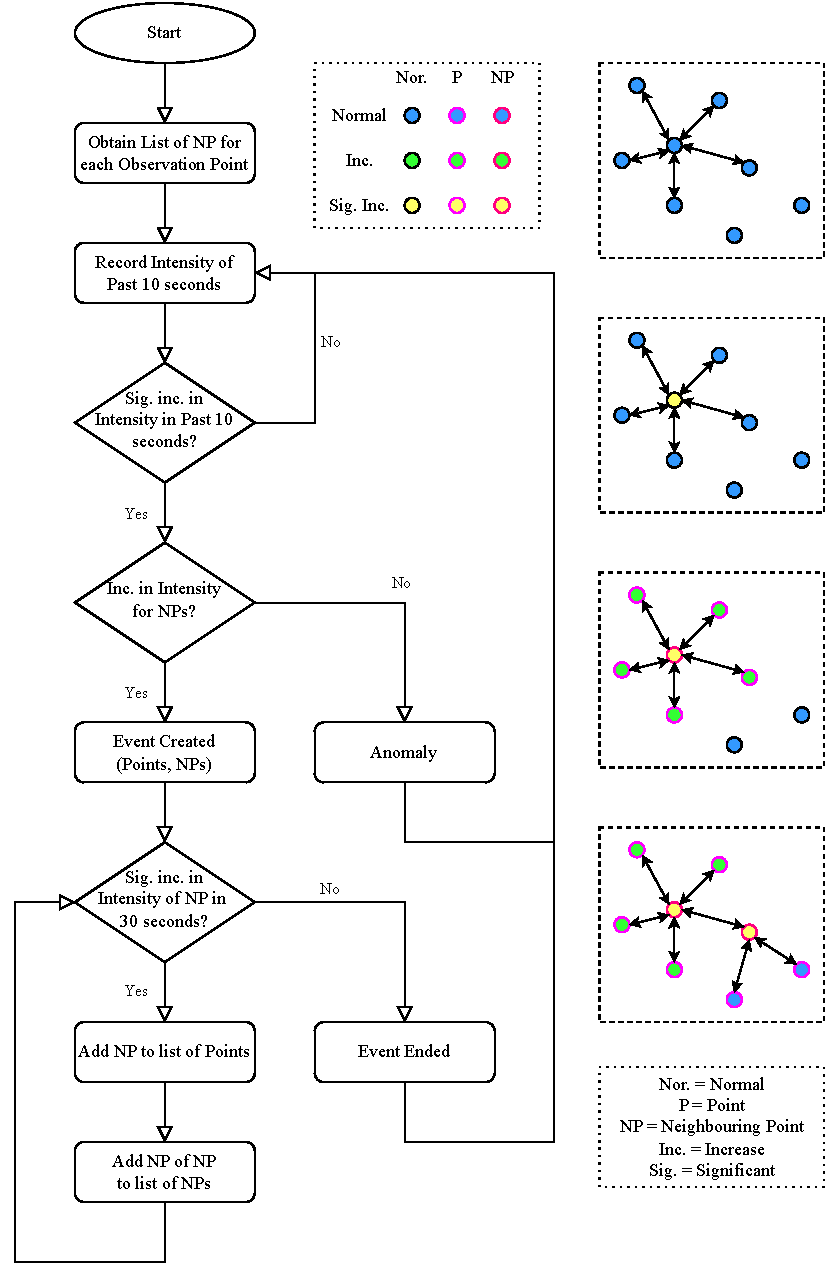
\includegraphics[width=0.8\linewidth]{shake-detection.pdf}
    \caption{Shake detection flowchart and diagram.}
    \label{fig:shake-detection-diag}
\end{figure}

This section referred to \href{https://qiita.com/ingen084/items/82985e8d3227c97c608d}{this blog article} written by Ingen.

\section{User Interface}

The GUI will be designed using Avalonia, which is designed to develop cross-platform applications in .NET.

The package MapsUI \autocite{mapsui-github} will be used to draw the maps in the application, since it is one of the best-supported candidates in .NET.

The nature of this application decided that the UI will be a graphical interface. Comparing MAUI in .NET with Avalonia, due to the fact that MAUI is more suitable for a mobile touch-based platform (that also works on desktop), while Avalonia is designed to support the desktop paradigm, the latter will be used to implement the graphical interface.

As discussed in the previous sections, there are three main pages that the program will include: the page for real-time observations, the page for viewing past earthquakes, and the page for controls and settings.

A sidebar is used to switch between the three pages.

Note that the following mock-up images are for demonstration purposes only -- it is not an actual earthquake.

\subsection{Real-Time Monitoring Screen}

The real-time monitoring screen holds the following three functionalities:
\begin{itemize}
    \item real-time intensity display (including shake detection boxes);
    \item tsunami warning display; and
    \item EEW display (including predicted intensity colouring and real-time wavefront positions).
\end{itemize}

\begin{figure}[htp]
    \centering
    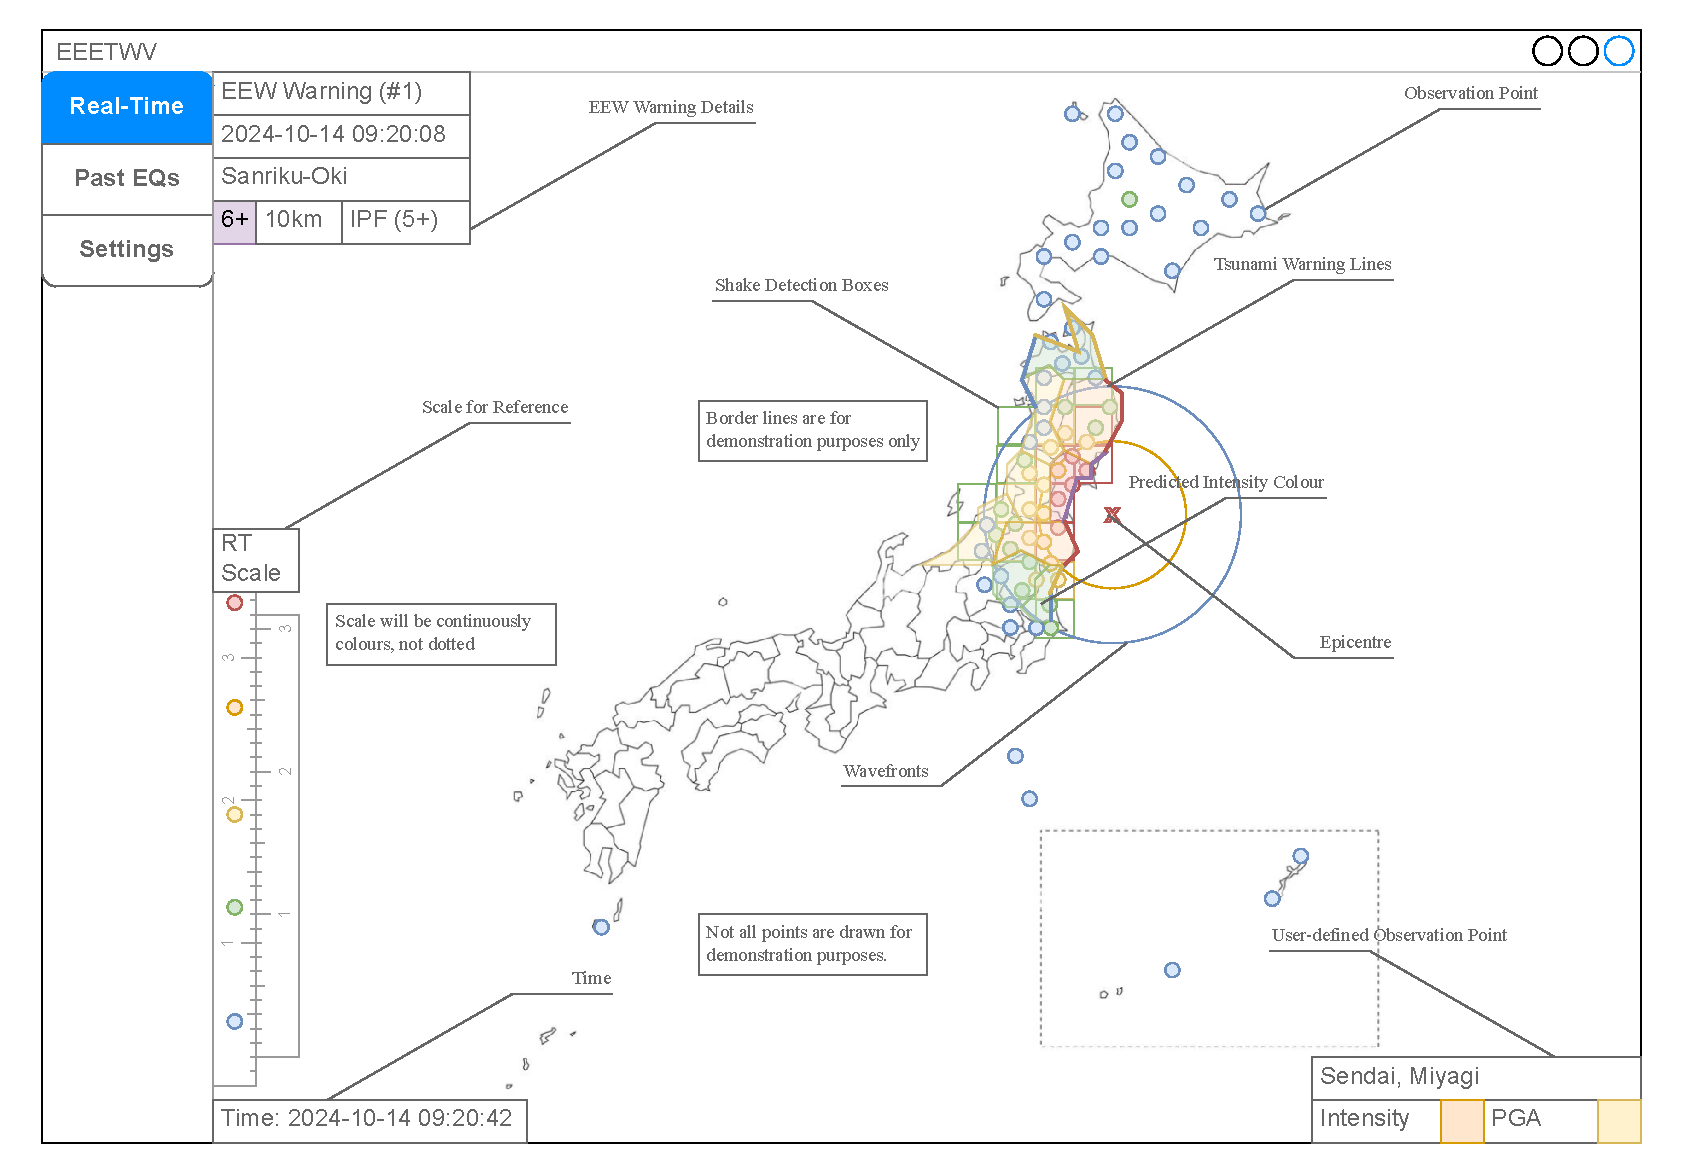
\includegraphics[width=\linewidth]{gui-mockup-rt.pdf}
    \caption{Design of GUI for Real-Time Page.}
    \label{fig:gui-mockup-rt}
\end{figure}

Figure \ref{fig:gui-mockup-rt} shows a design of this page that will be implemented. The real-time intensity colour points, the current time and the colour scale will be displayed at all times.

The shake detection boxes will only be displayed when there is shake detected as described in the algorithm section, and would be coloured into red, yellow or green in accordance to the intensity of the event.

The tsunami warning will be displayed only if it is released (or updated). It will consistently flash at 0.5 Hz to warn the users and to signify its presence.

The EEW warning display will only be present when an EEW is ongoing, until 1 minute after the final EEW warning. The top-left box will display key properties of the earthquake (including the predicted maximum intensity in the corresponding colour), with relatively smaller text displaying the details, such as the shake detection algorithm used (e.g. IPF/PLUM etc.). The map will be coloured in accordance to the predicted intensities released in the EEW.

There are no buttons or interactions for the user to interact with. However, this page will have a relatively high refresh rate to ensure that the data displayed is up-to-date.

\subsection{Past Earthquakes}

The past-earthquake screen regularly displays a sidebar to select the earthquake from, with by default the latest earthquake selected, with a map in the middle. Figure \ref{fig:gui-mockup-pe} shows a design of this page.

\begin{figure}[htp]
    \centering
    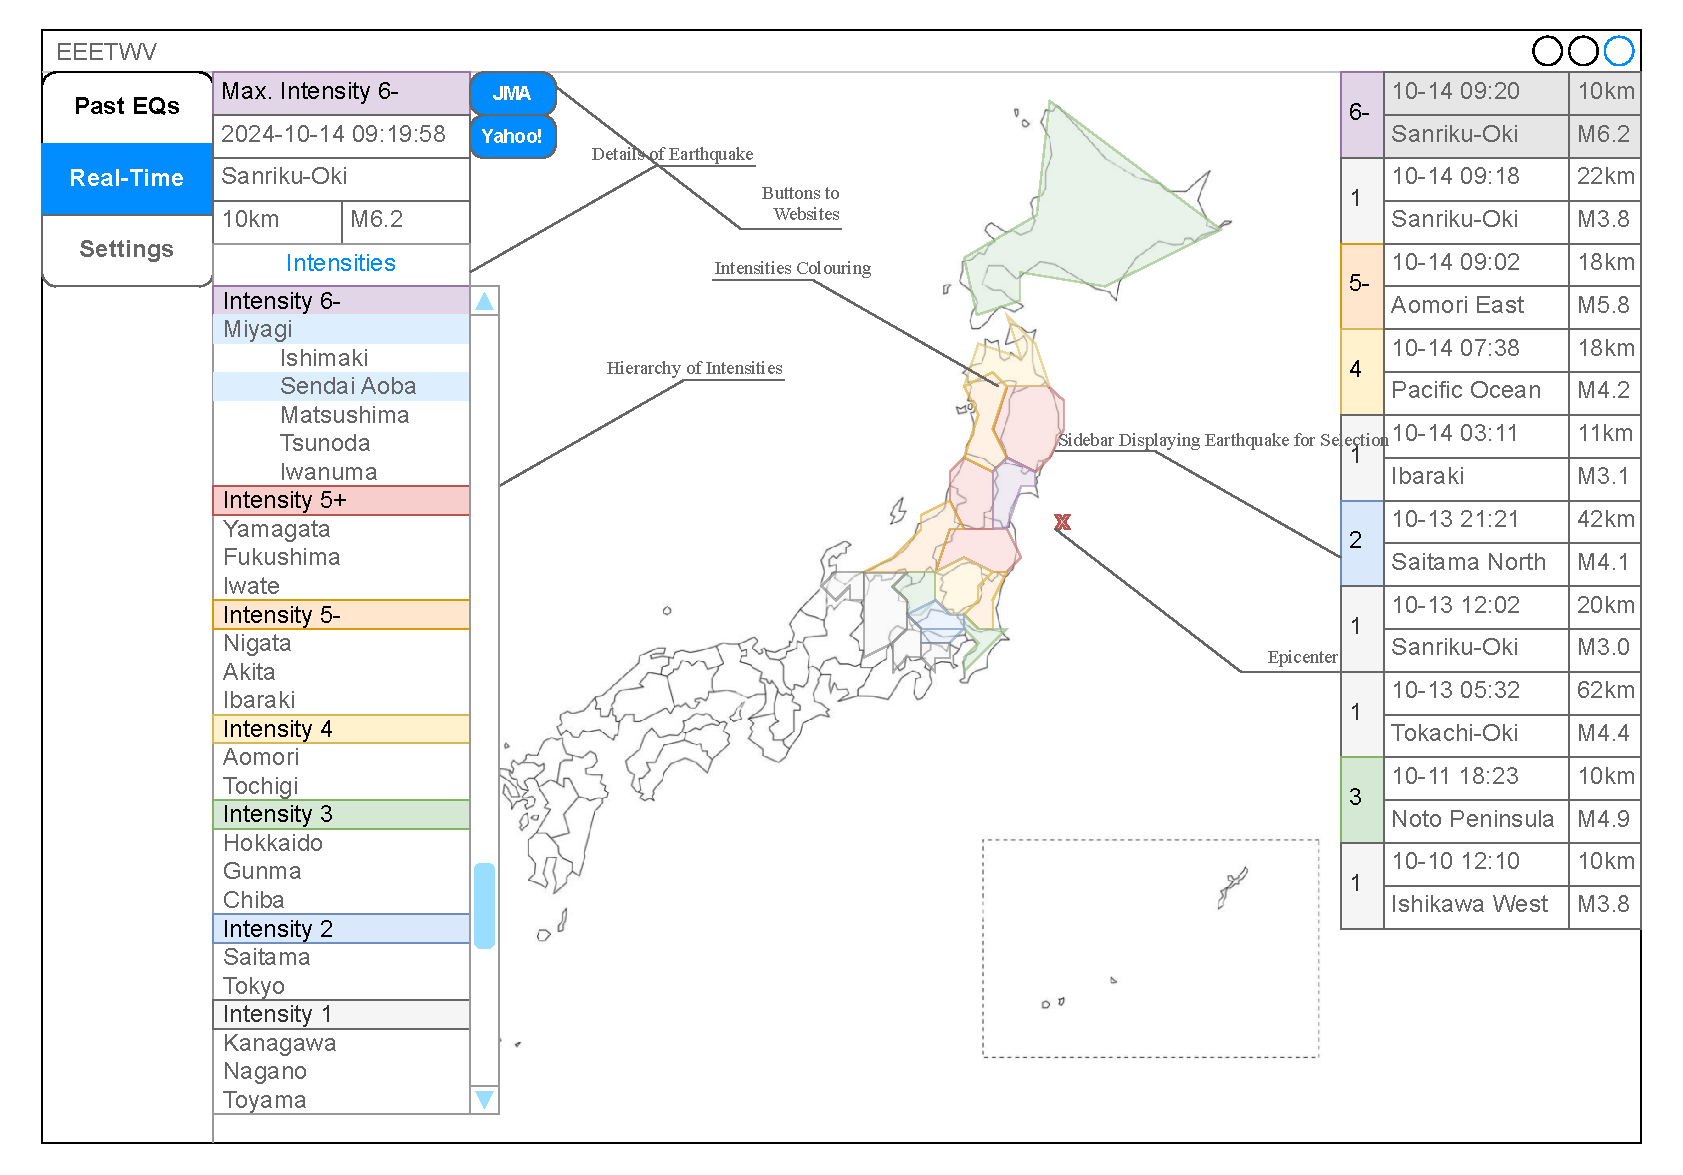
\includegraphics[width=\linewidth]{gui-mockup-pe.pdf}
    \caption{Design of GUI for Past Earthquakes Page.}
    \label{fig:gui-mockup-pe}
\end{figure}

For each earthquake, the sidebar should display the time of the earthquake, the epicentre of the earthquake (position and depth), the maximum intensity of the earthquake (in the correct corresponding colour), and its magnitude.

In the centre, there should be a map colouring the observed intensity of the earthquake, together with a cross to indicate the position of the epicentre.

On the left, there should be the details displayed in a bigger font, and an expandable sidebar to see the intensity of each observation point, in a hierarchy according to the province and the county. There should be two buttons, one corresponding to the JMA website to view the details, and another to jump to a weather service provider to view the details of the earthquake.

\subsection{Customisation Page}

In the customisation page, there should be a place to input an API Key from DM-D.S.S., and in the future this should be upgraded to a button to provide a login using OAuth 2 and the default browser.

There should also be a page to customise sound files for different events, a page to customise the intensity colour scheme, and to define a key point on the map to observe the intensity.

Figure \ref{fig:gui-mockup-customisation} shows a mock-up of the design of the customisation page.

\begin{figure}[htp]
    \centering
    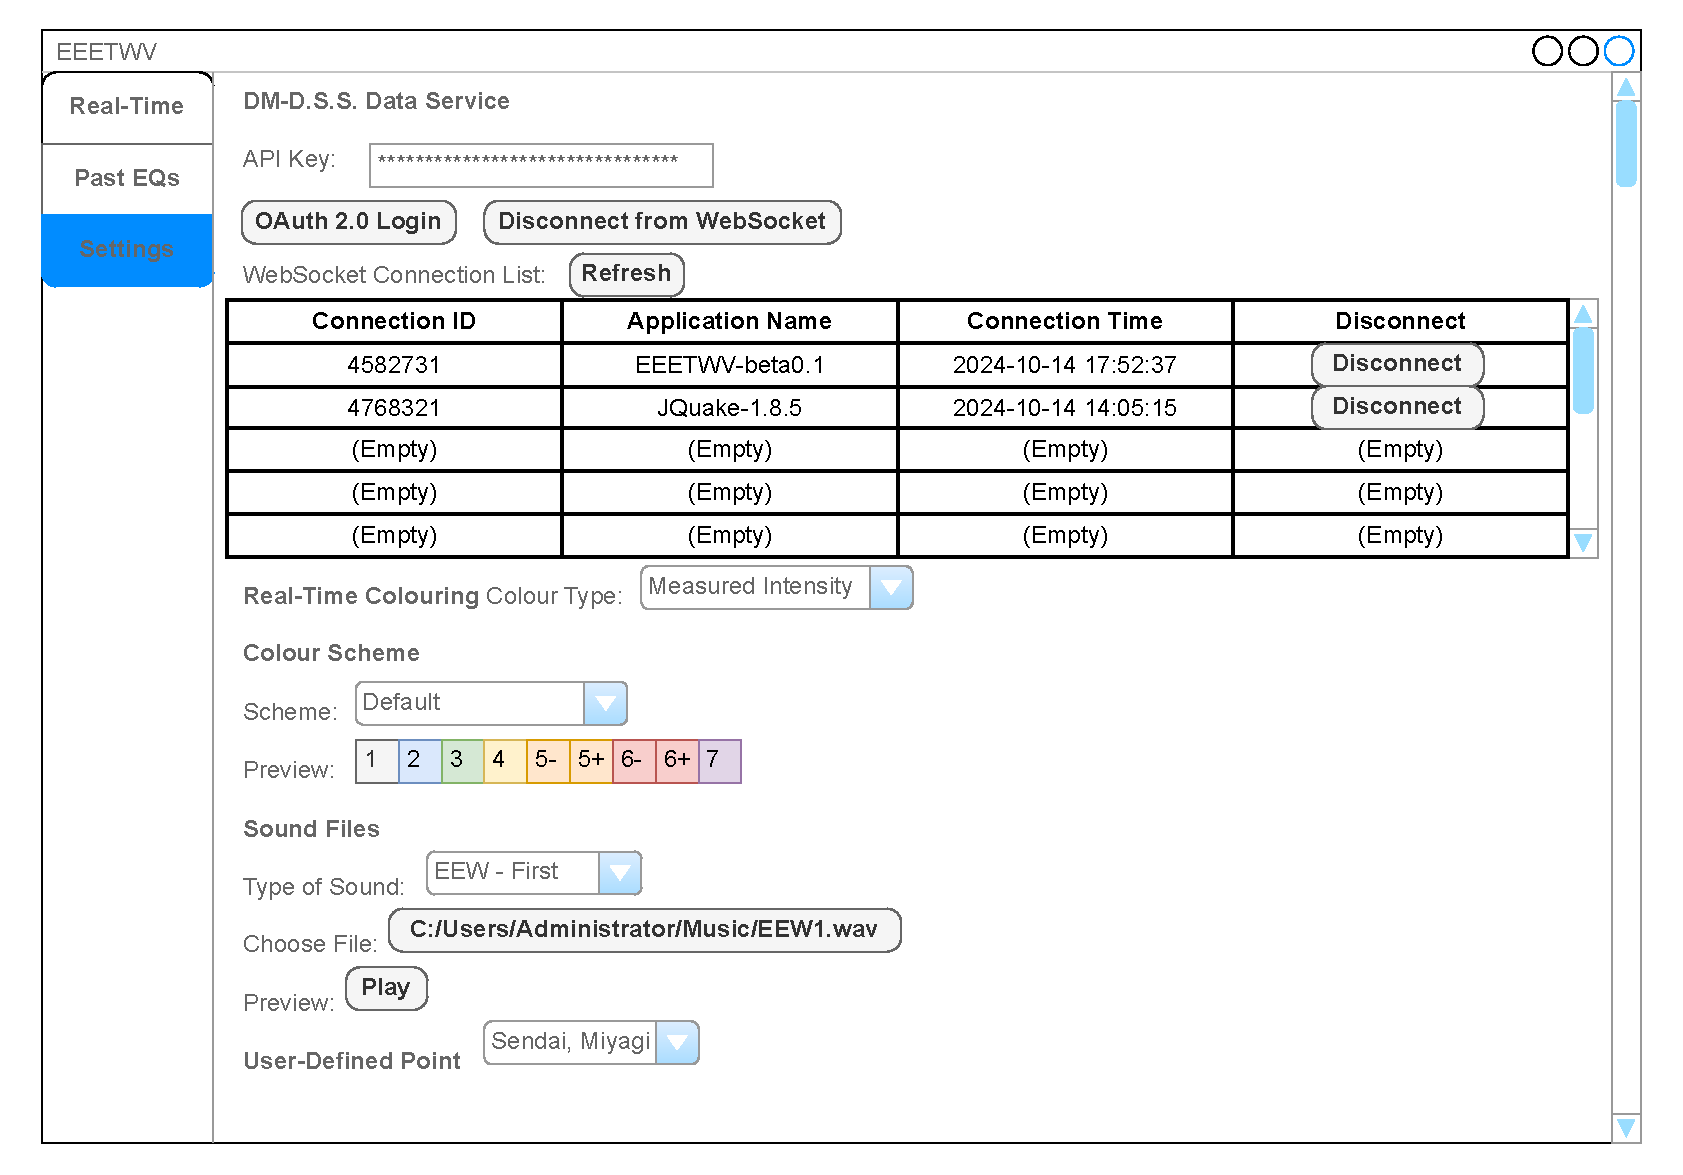
\includegraphics[width=\linewidth]{gui-mockup-customisation.pdf}
    \caption{Design of GUI for Customisation Page.}
    \label{fig:gui-mockup-customisation}
\end{figure}

\subsection{Joint Functionalities and Technicalities}

There is a joint functionality between the real-time page and the past earthquakes page, that is, when a new EEW/Tsunami Warning is released, the application should automatically jump to the real-time page to display the latest earthquake information to the user.

Since this a GUI-based application, there will be a significant use of asynchronous programming and events. Specifically, EEWs should be treated as events for the GUI application to handle and display, and user inputs are also events that the program should respond to.

\ToDo{Talk about events more}

% TODO: Talk about events more

\section{OOP Model}

\subsection{Design Patterns}

\subsection{Abstractions (Interfaces, Options) and Services (Classes)}

\subsection{Design of DTOs (Record Classes)}

\ToDo{Finish up class diagram with text explanation}

% TODO: Finish OOP

The data achieved by the previous two data sources will be parsed into objects (classes, records) to transfer between different components of the program. Those objects will then be transferred to the GUI component and be displayed.

The data achieved using the NIED Kyoshin Monitor (observation points) will be converted into objects. The class diagram is shown in is shown in Figure \ref{fig:classes-kmoni}.

\begin{figure}[htp]
    \centering
    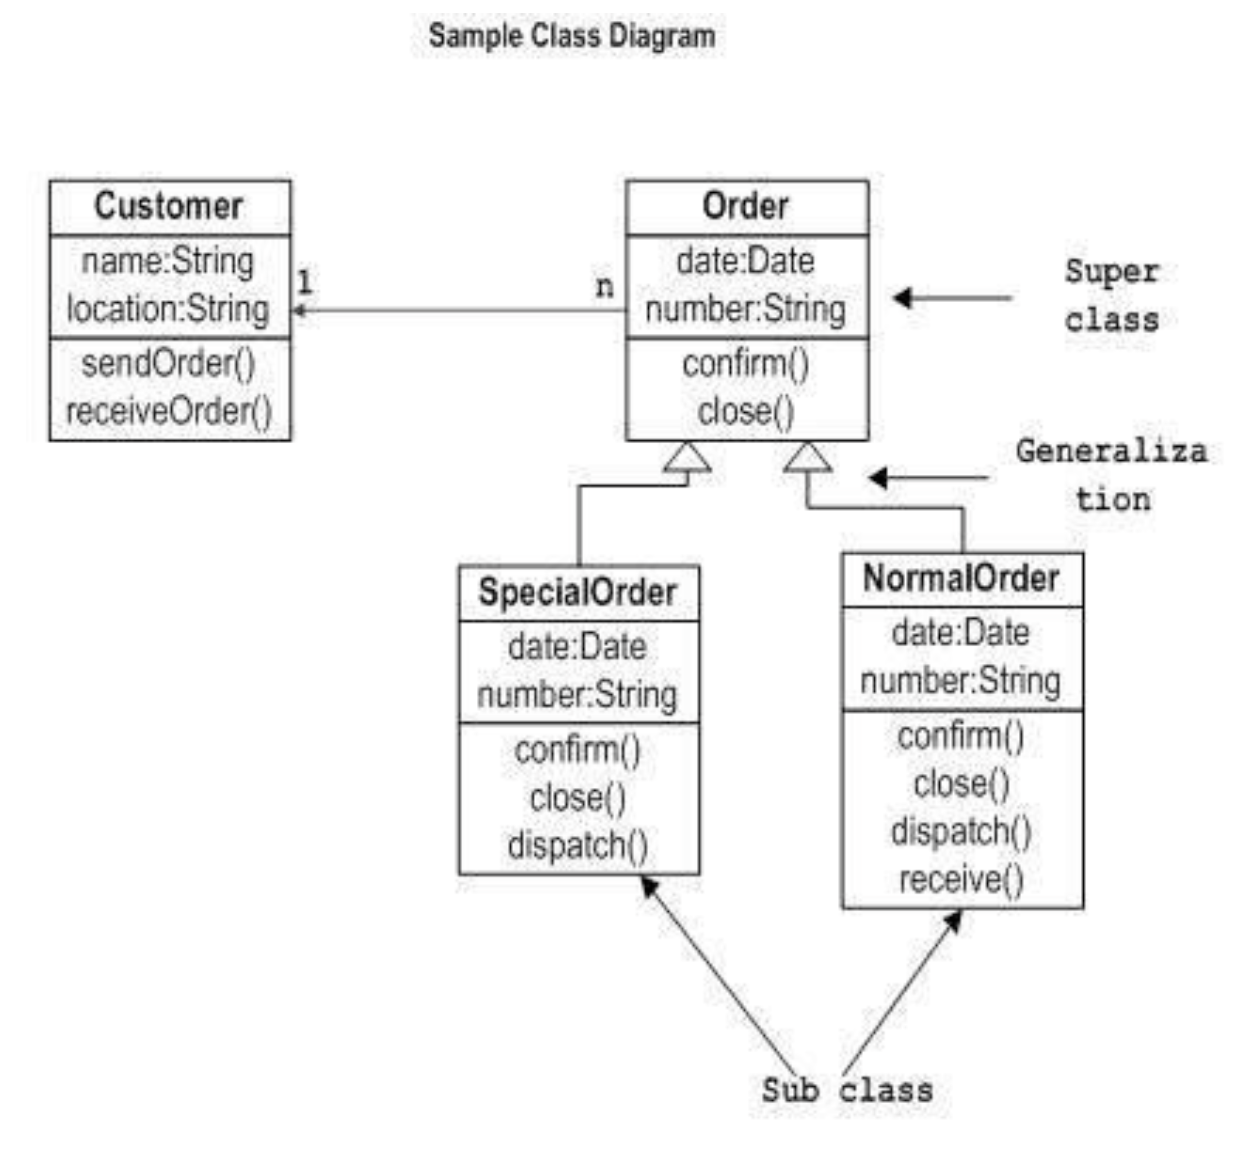
\includegraphics[width=0.5\linewidth]{class_diagram.png}
    \caption{Class Diagram for Kyoshin Monitor data objects}
    \label{fig:classes-kmoni}
\end{figure}

The GIF images will be parsed with the built-in \Code{SkiaSharp} module by mono, which could also be used to draw the map.

The class diagram following the UML convention for the HTTP-based API calls is shown in Figure \ref{fig:classes-http}. The JSON responses will be converted to C\# objects using \Code{System.Text.Json} modules.

\begin{figure}[htp]
    \centering
    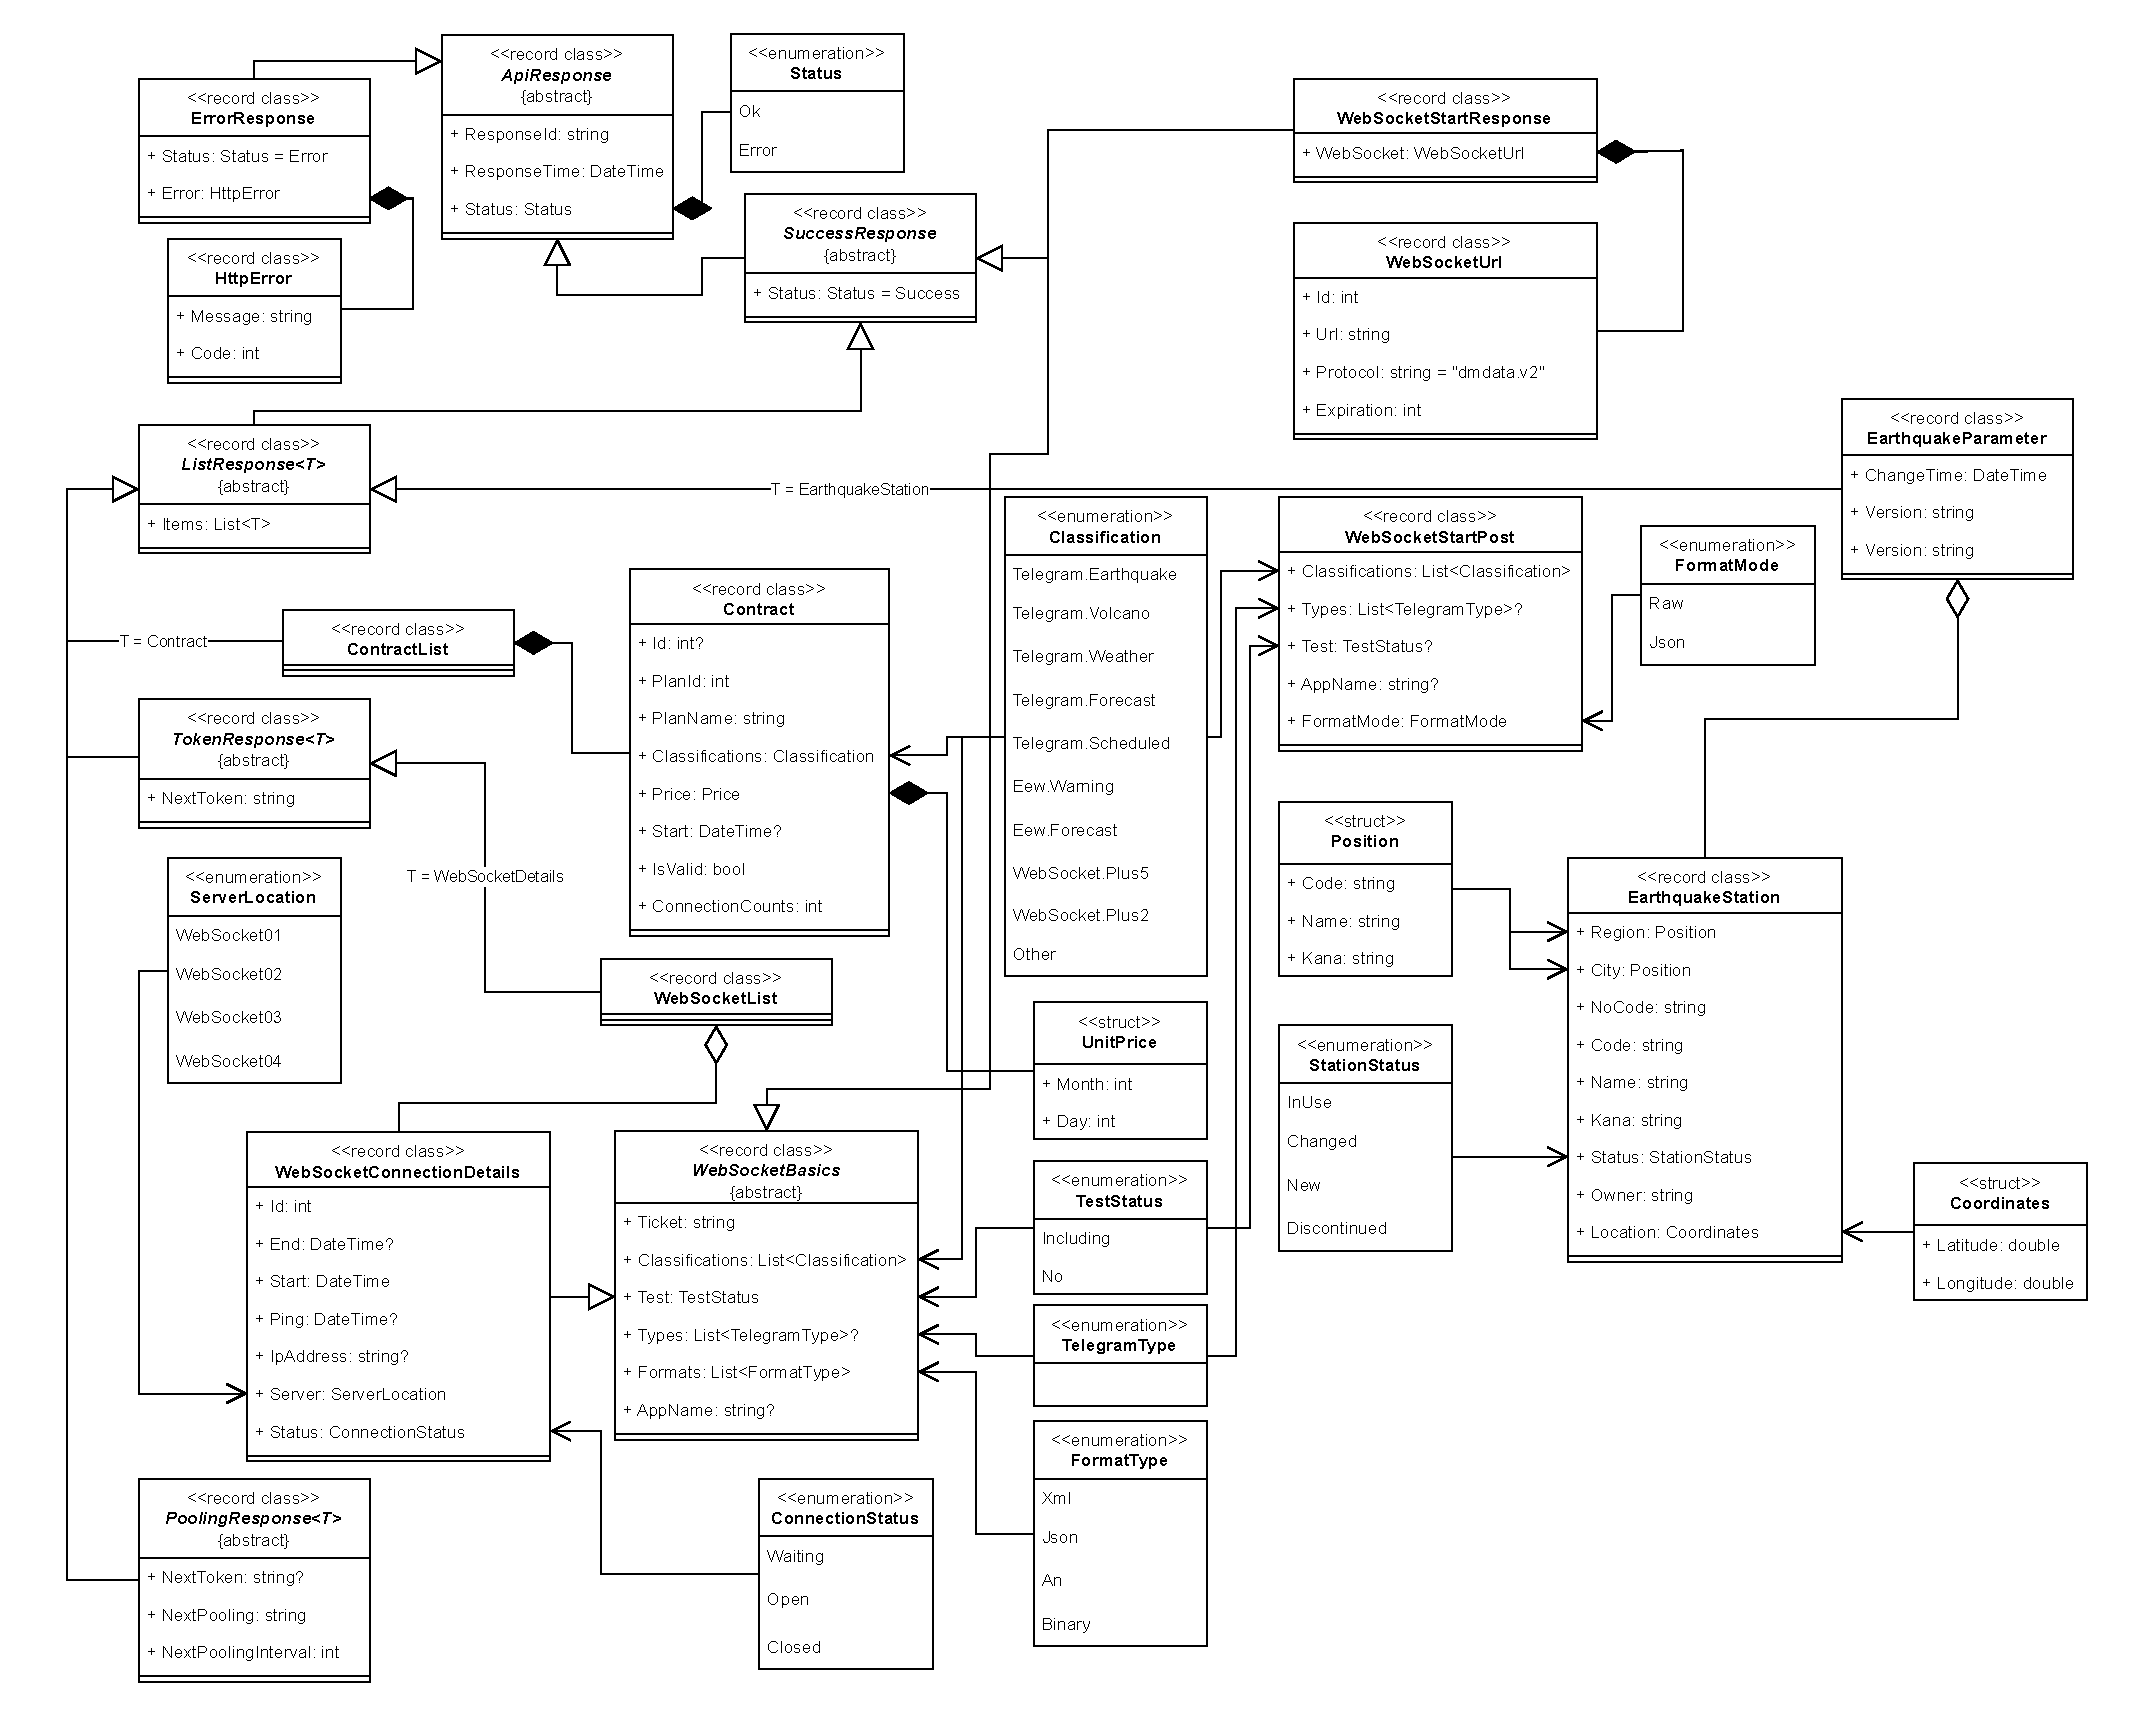
\includegraphics[width=\linewidth]{class-http.pdf}
    \caption{Class Diagram for HTTP data objects}
    \label{fig:classes-http}
\end{figure}

This shows the use of composition and inheritance. The use of generics is also demonstrated.

The class diagram for the WebSocket based calls is shown in Figure \ref{fig:classes-ws}.

\begin{figure}[htp]
    \centering
    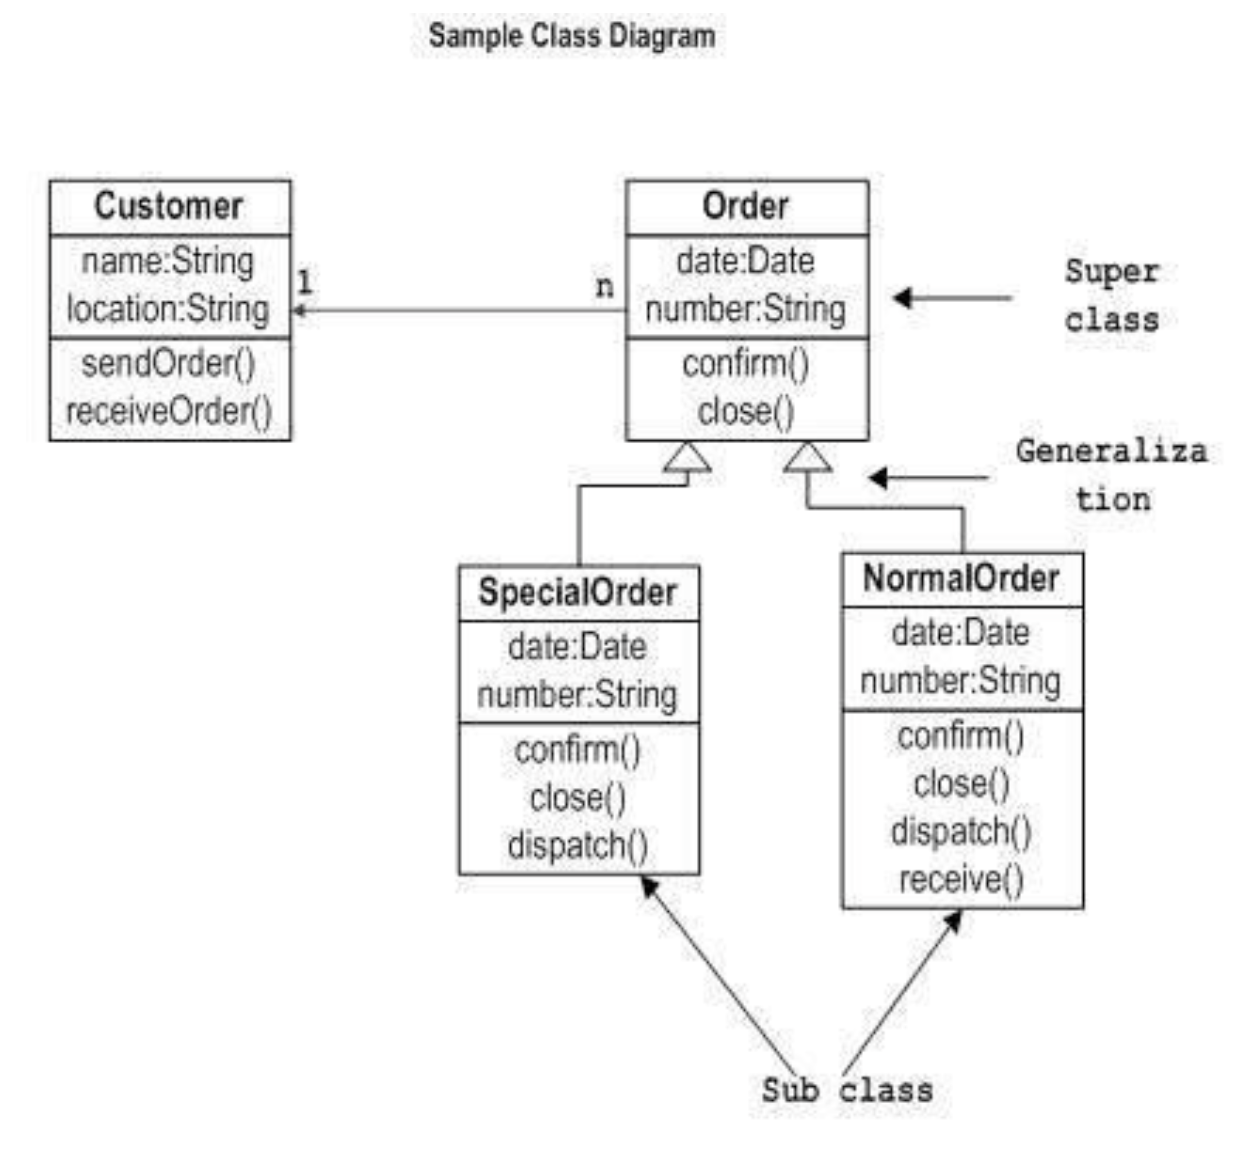
\includegraphics[width=0.5\linewidth]{class_diagram.png}
    \caption{Class Diagram for WebSocket data objects}
    \label{fig:classes-ws}
\end{figure}

\subsection{The MVVM Pattern}

\section{Hardware \& Software Requirements}

Table \ref{tab:hardware-spec} outlines basic hardware requirements for the application.

\begin{table}[htp]
    \centering

    \begin{tabular}{|c|c|c|}
        \hline
        Type               & Minimum                        & Recommended                     \\
        \hline
        RAM                & 4 GB                           & 8 GB                            \\
        Storage Space      & 1 GB                           & 2 GB                            \\
        CPU                & Intel Core 8th Gen (or equiv.) & Intel Core 10th Gen (or equiv.) \\
        Display Resolution & 720p                           & 1080p                           \\
        Display Size       & 9''                            & 12''                            \\
        \hline
    \end{tabular}
    \caption{Hardware Specification for App}
    \label{tab:hardware-spec}
\end{table}

The amount of RAM is due to the amount of data that is processed (and considering other applications running as well). Storage space is not a substantial requirement of this application, while the CPU has to be of high standards to process all the data. To display the application properly (with appropriate size), a display of 1080p 12'' is recommended.

It will be able to run on up-to-date Windows, macOS and Linux distributions (both x64 and ARM) due to the cross-platform nature of .NET, but x86 platforms will not be supported.

The author uses a macOS 15 (beta) machine with 2.5K 13'' display, Intel Core i5-1038NG7 (with Intel Iris Plus Graphics) and 16 GB of RAM (MacBook Pro 2020, 4 Thunderbolt Ports) and a Windows 11 (beta) machine with 2.5K 15'' display, AMD Ryzen 7 5800H and 32 GB of RAM (with RTX 3070 for Laptop) (Legion R9000K 2021) to test the application, and with 2.5K 24'' external display as well. An Ubuntu 22.04 virtual machine will be used to test the compatibility for Linux systems.

The application will be self-contained (i.e. comes with .NET runtime) to prevent the user from unnecessary technical complications.

The device needs to have stable connection to the internet using Wi-Fi/Ethernet/other means, to establish connection with the relevant APIs.